\documentclass[11pt]{article}
\usepackage[utf8]{inputenc}
\usepackage[T1]{fontenc}
\usepackage{amsmath, amsfonts, amssymb, amsthm}
\usepackage[numbers,sort&compress]{natbib}
\usepackage{mathtools}
\usepackage{geometry}
\geometry{margin=1in}
\usepackage{tikz-cd}
\usepackage{float}
\usepackage{placeins}   % for \FloatBarrier
\usepackage{caption}    % nicer caption control
\captionsetup[figure]{font=small,labelfont=bf}
\usepackage{enumitem}
\usepackage[hidelinks]{hyperref}
\usepackage{orcidlink}
\usepackage{cleveref}
\usepackage[final]{microtype}
\usepackage{csquotes}

% Typography improvements
\setlength{\emergencystretch}{3em}
\numberwithin{equation}{section}
\allowdisplaybreaks

% Theorem environments

% === Theorem environments (uniform upright) ===

\newtheoremstyle{upright}%
  {3pt}{3pt}%   Space above/below
  {\normalfont}% Body font (upright)
  {}%           Indent amount
  {\bfseries}%  Head font
  {.}%          Punctuation after head
  {.5em}%       Space after head
  {}%           Head spec

\theoremstyle{upright}

\newtheorem{theorem}{Theorem}
\newtheorem{lemma}{Lemma}
\newtheorem{corollary}{Corollary}
\newtheorem{proposition}{Proposition}
\newtheorem{definition}{Definition}
\newtheorem{remark}{Remark}
\newtheorem{example}[theorem]{Example}

% Custom commands
\newcommand{\V}{\mathcal{V}}
\newcommand{\Prof}{\mathrm{Prof}}
\newcommand{\ProfV}{\Prof_{\V}}
\newcommand{\Lan}{\mathrm{Lan}}
\newcommand{\Ran}{\mathrm{Ran}}
\newcommand{\profto}{\rightsquigarrow}
\DeclareMathOperator{\Hom}{Hom}
\newcommand{\BC}{Beck--Chevalley}
\newcommand{\resid}{\multimap}
\newcommand{\gapV}{\operatorname{gap}_{\V}}
\newcommand{\R}{\mathbb{R}}
\newcommand{\adj}[2]{\ensuremath{#1 \dashv #2}}
\newcommand{\Sh}{\mathrm{Sh}}


% Title and author information
\title{Quantifiers, Composition, and Convexity: An Associahedral/Day Calculus for Optimization}
\author{Lorand Bruhacs\,\orcidlink{0009-0004-6751-0715}}
\date{\today}

\begin{document}

\maketitle

\begin{abstract}
We recast optimization with quantifier alternation in the language of enriched Kan extensions and residuation, and extend this calculus to \emph{compositional} pipelines. Our main identity encodes a $\forall\exists$ alternation as a single $\exists$ with a residual profunctor in the biclosed bicategory $\V\text{-}\Prof$. We show when Beck--Chevalley (BC) exactness upgrades this compilation to an equality and prove a one–shot BC/Sion theorem in barycentric enrichments. The new contribution is a compositional layer: we index regroupings of modules by the \emph{associahedra} and endow presheaves over the bracketing category with \emph{Day convolution}. A tensor–stable sheafification then acts as a lax–monoidal “associahedral convex hull,” yielding: (i) \emph{rebracketing invariance} (BC along associahedral faces), (ii) \emph{quantifier pushforwards} by residuation through Day kernels, and (iii) \emph{one–shot} minimax equalities that persist under composition. Operationally, bilevel robust/ adversarial objectives collapse to single envelopes that are independent of how subsystems are grouped, with failure localized as horn fillers on the associahedron. We illustrate compiled residuals in conic/ellipsoidal modalities, giving single SOCP/SDP formulations that replace inner oracles.
\end{abstract}

\tableofcontents

\section{Introduction}
\label{sec:intro}

Modern optimization is a success story of craft and context. Practitioners assemble bespoke pipelines—line searches, proximal steps, robust penalties, adversarial inner loops—tailored to data and compute. This craft delivers results, but it also obscures structure: why do some pipelines compose cleanly while others become brittle? When does a nested min--max reduce to a single solve, and when does it not? How should we reason about an objective that is built from many modules whose grouping and order are chosen for convenience rather than principle?

Our point of view is that these questions are best answered by separating \emph{logic} from \emph{geometry}. The logic of an optimization pipeline is its pattern of quantifiers (``there exists a step'', ``for all perturbations'', ``exists--for all--exists'' in multi-stage games). The geometry is the medium in which these quantifiers act: costs, penalties, divergences, transport, norms—encoded by an \emph{enrichment} $\V$ that determines how we measure, combine, and compare values. Once this separation is made, many familiar constructions appear in a common mirror: left Kan extensions (existentials) for optimistic aggregation, right Kan extensions (universals) for conservative envelopes, and their interaction governed by standard exactness conditions. The quantifier pattern reflects the logical complexity of the optimization procedure~\cite{Lawvere1973,Kelly1982}.

This lens already explains basic moves. A line search that chooses an admissible step by a sufficient-decrease test is an \emph{existential} aggregation over a poset of step sizes; a robust envelope that certifies progress against an uncertainty class is a \emph{universal} aggregation over perturbations. Crucially, both are \emph{weighted} by the geometry $\V$: in a min--plus base they are infimal/supremal convolutions; in an optimal-transport base they are Kantorovich-style envelopes; in information geometry they become entropic or $\phi$-divergence surrogates. This unifies many ``tricks'' as instances of the same two operations.

Real pipelines, however, are not single moves but \emph{compositions} of moves. We precondition, then linearize, then regularize, then robustify, and so on. In practice the grouping and order of these modules is often chosen for numerical convenience, even though associativity only holds \emph{up to} modeling error. This raises a structural demand: the value of a compiled objective should not depend on how we parenthesize a fixed list of modules. In other words, we need a rebracketing story. The combinatorics of rebracketing is organized by the \emph{associahedron} in the sense of Stasheff and Loday~\citep{Stasheff1963I,Loday2004}, and the corresponding algebra on presheaves is a Day convolution~\citep{Day1970}—the canonical way to ``multiply'' a module kernel induced by composition. 

The first contribution of this paper is a compact identity—an \emph{Alternation Lemma}—that compiles a universal–after–existential pattern into a single existential weighted by a \emph{residual} kernel. Under standard Beck--Chevalley exactness in a barycentric base, this becomes a genuine equality and \emph{subsumes familiar minimax exchanges}. Concretely, in the KR/Wasserstein--1 geometry, for any $L$–Lipschitz payload $h$ we recover the Kantorovich–Rubinstein~\cite{Villani2009} residual
\[
\sup_{\mathsf P:\,W_1(\mathsf P,\widehat{\mathsf P})\le \rho}\ \mathbb E_{\mathsf P}[h]
\;=\;\mathbb E_{\widehat{\mathsf P}}[h]\;+\;\rho\,L
\quad\Longleftrightarrow\quad
Q\resid P=\big(a\mapsto \mathbb E_{\widehat{\mathsf P}}[h(a,\cdot)]+\rho L_a\big),
\]
and in the conic/ellipsoidal setting we recover the \emph{support–function} residuals and the \emph{S–lemma}~\cite{PolikTerlaky2007} as categorical instances:
\[
\sup_{\|C b\|_2\le \rho}\ \langle s(a),b\rangle
\;=\;\rho\,\|C^{-T}s(a)\|_2
\quad\text{(SOCP)},\qquad
\sup_{\|C b\|_2\le \rho}\ \Big(r(a)+\tfrac12 b^\top H(a)b+\langle s(a),b\rangle\Big)
\ \overset{\mathrm{S\text{-}lemma}}{=}\ \text{SDP}.
\]
(Analogous closed forms arise for $\phi$–divergence balls via Fenchel duals.) The second contribution is \emph{compositional}: we equip presheaves over the bracketing category with Day convolution and introduce an associahedral convex hull $\mathsf{cl}$ that is lax–monoidal. This yields two guarantees: (i) compiled values are \emph{rebracketing–invariant} after closure (associahedral BC), and (ii) “convexify–then–compose’’ is never stronger than “compose–then–convexify’’ (a Minkowski–type subadditivity for pipelines).

The practical payoff is straightforward. Residualizing each module once and composing via Day turns bilevel and multistage objectives into \emph{single} envelopes, independent of grouping. In conic/ellipsoidal modalities this produces one SOCP/SDP per instance (no inner oracles, no inner--outer tolerance coupling) and exposes \emph{diagnostics}: any remaining gap before closure localizes to specific faces of the associahedron (``horns''), pinpointing exactly which module interfaces violate convexity or continuity assumptions. The result is a principled path from modular design to certifiable envelopes—without sacrificing the engineering flexibility that motivates modular pipelines in the first place.

\paragraph{From Armijo to left--Kan along admissible morphisms.}

As a concrete anchor, consider Armijo backtracking~\cite{NocedalWright2006}): accept $\alpha>0$ along $d$ if
\[
f(x+\alpha d) \le f(x)+c\,\alpha\,\nabla f(x)^\top d \qquad (0<c<1).
\]
This already hints at the categorical viewpoint. Regard \emph{states} as objects of a (pre)ordered category and \emph{updates} $x\to x+\alpha d$ as morphisms. The Armijo inequality acts as a \emph{lax constraint} selecting \emph{admissible morphisms}. The prescription \enquote{pick the largest admissible $\alpha$} is then an \emph{order-enriched colimit} over the step poset; in \S\ref{sec:math-framework} we will see this is the $\Sigma_1$ case of our general picture via a left Kan extension along a feasibility/penalty profunctor.

\paragraph{A matching right--Kan example: conservative envelopes via optimal transport.}
Recall that for a profunctor $P:A\profto X$ and a $\V$--functor $F:A\to\V$,
\[
\Ran_{P}F(x)\;=\;\int_{a\in A}\,[\,P(a,x),\,F(a)\,].
\]
In the min--plus base $\V=(\overline{\mathbb R},\ge,+,0)$, the internal hom is subtraction, so
\[
\Ran_{P}F(x)\;=\;\sup_{a\in A}\ \big\{\,F(a)\;-\;P(a,x)\,\big\},
\]
i.e.\ a \emph{conservative} bound: the largest value guaranteed after paying the penalty $P$.

\medskip
\noindent\emph{OT as a profunctor.}
Model \emph{step candidates} by $A$ and \emph{states} by $X$. For each $a\in A$ (e.g.\ a step size/direction), let $\mu_a$ be a predictive law for next--state outcomes (from a local model or stochastic oracle). For each $x\in X$, let $\nu_x$ be a nominal/target law (e.g.\ $\delta_{x}$, or a fitted distribution for the realized update). Define the profunctor $P$ by an optimal transport cost,
\[
P(a,x)\;:=\;W_c(\mu_a,\nu_x),
\]
such as the Wasserstein--1 distance $W_1$ for ground cost $c$. Then
\[
\boxed{\quad
\Ran_{P}F(x)\;=\;\sup_{a\in A}\ \Big\{\,F(a)\;-\;W_c(\mu_a,\nu_x)\,\Big\}.
\quad}
\]
Here $F(a)$ is the predicted improvement (e.g.\ modelled decrease), and $W_c(\mu_a,\nu_x)$ penalizes the geometry/data mismatch between the model’s outcome law and what the state $x$ actually induces.

\medskip
\noindent\emph{Dual reading (Kantorovich).}
For $W_1$, $W_1(\mu_a,\nu_x)=\sup_{\|\varphi\|_{\mathrm{Lip}}\le 1}\ \mathbb E_{\mu_a}[\varphi]-\mathbb E_{\nu_x}[\varphi]$. Plugging this into the display shows that $\Ran_{P}F(x)$ is the \emph{best guaranteed envelope} after accounting for all $1$--Lipschitz probes that measure how far the local prediction can be transported to reality.

\medskip
\noindent\emph{Line search interpretation.}
Where Armijo/\(\Lan\) is \emph{optimistic} (“find a feasible step with sufficient modeled decrease”), the OT/\(\Ran\) envelope is \emph{conservative}:
\[
\text{choose }a^\star\in\arg\max_{a\in A}\ \Big\{\,F(a)-W_c(\mu_a,\nu_x)\,\Big\},
\]
i.e.\ pick the step that maximizes the decrease you can \emph{guarantee} even if the geometry warps under the transport from prediction to realization. This pairs with the Armijo example as the $\Pi_1$ counterpart and sets up the $\Ran\!\circ\!\Lan$ patterns treated later.

\subsection{The Categorical Perspective}

At a technical level, our main contribution is a compact identity in enriched category theory:
\begin{equation}\label{eq:main-identity}
\Ran_Q(\Lan_P F) \cong \Lan_{Q \multimap P} F,
\end{equation}
where $(Q \multimap P)(a,x) = \int_b [Q(b,x), P(a,b)]$ is the \emph{right residual} of profunctors $P$ and $Q$. This identity exhibits the \emph{biclosedness} of the bicategory $\V\text{-}\Prof$ and provides a computationally effective pointwise formula via ends and coends. The pointwise calculation uses Fubini for enriched (co)ends~\cite{Dubuc1970}.

\paragraph{Why this identity matters.}
Equation~\eqref{eq:main-identity} is not an isolated trick: it is the expression of the \emph{biclosedness} of $\V\text{-}\Prof$ in the language of Kan extensions. It says a universal step followed by an existential step \emph{compiles} into a single existential step with a \emph{residual} weight; this is the formal backbone of \enquote{minimax = maximin} and related reformulations under exactness. 

\paragraph{Alternation (quantifier exchange).}
Under standard Fubini for (co)ends and exactness (Beck--Chevalley), the alternation law
\[
\Ran_Q(\Lan_P F) \cong \Lan_{Q\multimap P} F
\]
(\Cref{eq:main-identity}) replaces ``$\forall$ then $\exists$'' by a single $\exists$ with \emph{residual} weight
\[
(Q\multimap P)(a,x) = \int_{b}[Q(b,x), P(a,b)].
\]
Operationally: scope exchange is legal exactly when the square is exact (BC). We further show that these results are \emph{composition-invariant}: using Day convolution over an associahedral indexing of parenthesizations, our one-shot reformulations do not depend on how subsystems are grouped. For BC in categorical logic and hyperdoctrines, see \cite{Seely1983,Jacobs1999}.

\subsection{Relationship to Existing Literature}

We should clarify what is new in our approach versus what is established in the categorical logic literature. The mathematical content of our Alternation Lemma is essentially the \emph{Beck--Chevalley condition combined with Fubini theorems for enriched ends and coends}—results that are well-established in categorical logic, though not typically phrased in optimization language.

The correspondence between quantifiers and Kan extensions is well established in the enriched setting:
\begin{itemize}[itemsep=0.5ex]
\item In \citet{Lawvere1973}, ends and coends in Lawvere metric/enriched categories are read as
      $\forall/\exists$ quantifiers over enriched structure.
\item In \emph{hyperdoctrines}, quantifiers arise as adjoints to substitution, paralleling
      $\Lan/\Ran$ as adjoints to precomposition: see \citet{Lawvere1969} and
      \citet{Seely1983}, and the systematic account in \citet{Jacobs1999}.
\item For the 2-categorical calculus behind our use of mates and Kan extensions, see
      \citet{StreetWalters1978} and the enriched treatment in \citet{Kelly1982}.
\item Bicategorical/proarrow viewpoints (distributors, equipments) make
      $\Lan_P \dashv (-)\circ P \dashv \Ran_P$ explicit; cf.\ \citet{Benabou1967,Wood1990,Shulman2008}.
\end{itemize}


Thus, the mathematical machinery we employ is \emph{folklore in categorical logic}. Our contribution lies not in discovering new categorical results, but in:
\begin{enumerate}[itemsep=0.5ex]
\item \textbf{Translating} these established categorical principles into optimization language and applications
\item \textbf{Identifying} the correspondence between optimization complexity (alternation patterns) and logical complexity (quantifier depth)  
\item \textbf{Developing} a systematic framework for applying categorical logic to algorithm design
\item \textbf{Connecting} abstract categorical constructions to concrete optimization problems and convergence certificates
\end{enumerate}

The novelty is interpretative and applied rather than purely mathematical—we are essentially arguing that optimization theory has been rediscovering categorical logic principles in specialized contexts, and that making this connection explicit enables systematic algorithm design.

\subsection*{Related work}
\paragraph{Categorical.}
Our use of enriched ends/coends and Kan extensions follows the standard references in enriched category theory, notably Kelly’s monograph \citet{Kelly1982}; the pointwise alternation steps rely on Fubini for enriched (co)ends \citep{Dubuc1970}. The biclosed structure behind $\V$-\textbf{Prof} and residuals traces back to Bénabou’s bicategories \citep{Benabou1967}, the 2-categorical Yoneda/Kan calculus of Street–Walters \citep{StreetWalters1978}, and subsequent proarrow/equipment frameworks (Wood’s proarrow equipment and Shulman’s framed bicategories) \citep{Wood1990,Shulman2008}. Quantifiers-as-adjoints and the Beck–Chevalley condition originate in the hyperdoctrine tradition (Lawvere, Seely) and are systematized in categorical logic \citep{Lawvere1969,Seely1983,Jacobs1999}. 

\paragraph{Geometric.}
On the geometric side, our enrichment choices connect to abstract convexity and probabilistic semantics. For optimal transport and Kantorovich–Rubinstein duality, see \citet{Villani2009}; for categorical probability and Bayesian inversion in Markov categories (which supply mixing, testing, and transport semantics compatible with our residualization), see \citet{Fritz2020Markov}. Work on convex/affine structure in categorical settings provides complementary foundations for the “barycentric” hypotheses used here \citep[e.g.][]{Fritz2009Convex, EdelmanJamison1985}. Finally, our compositional layer uses Day convolution \citep{Day1970} and associahedral indexing \citep{LodayRonco1998,Loday2004} to organize rebracketing; the one-shot minimax upgrade relies on Sion’s classical theorem \citep{Sion1958} together with enriched Beck–Chevalley as in \citet{Kelly1982}. 

\paragraph{Recent directions.}
Beyond classical sources, several recent directions resonate with our compositional
and convex viewpoints.  On the convex–categorical side, \citet{HaderiOkayStern2024}
develop an \emph{operadic theory of convexity} (convex sets as algebras over a PROP),
providing a modern account of convex structure and tensoriality that fits well with our
barycentric hypotheses.  In parallel, \citet{Stein2023} propose a \emph{compositional}
framework for convex analysis based on convex bifunctions, furnishing graphical/dual
reasoning tools that align with our residual envelopes. Further adjacent developments include convex/operadic treatments of contextuality
\citep{Kharoof2022}, which connect categorical convexity with probabilistic models.


\subsection{The Logical Reading}

What makes this identity conceptually potent is its \emph{logical interpretation}. In enriched settings, Kan extensions compute weighted (co)limits in the base category $\V$, which itself encodes the geometry of an optimization problem—costs, penalties, divergences, or order relations. Under this reading:
\begin{itemize}[itemsep=0.5ex]
\item \textbf{Left Kan extensions} behave as \emph{weighted existentials} (optimistic aggregation): "there exists a step that yields improvement with cost measured in $\V$."
\item \textbf{Right Kan extensions} behave as \emph{weighted universals} (conservative bounds): "for all perturbations/adversaries, guarantee at least this much performance."
\item The \textbf{Alternation Lemma} is the categorical analog of \emph{quantifier exchange}: a $\forall\circ\exists$ computation can be recast as a single $\exists$ with a residual weight.
\end{itemize}

\paragraph{Modality via enrichment.}
The enriching category $\V$ fixes the semantics of weighted quantifiers:
\begin{itemize}[itemsep=0.25ex]
\item $(\overline{\mathbb R},\ge,+,0)$ --- min-plus cost geometry,
\item Fisher--Rao --- information geometry (natural gradients),
\item Wasserstein/OT --- probability metrics (DRO, JKO).
\end{itemize}
These choices determine how we combine, compare, and bound objectives.

\paragraph{Data of a step rule.}
To make the categorical framework concrete, we need three pieces of data for any optimization step:

First, let $A$ be the $\V$-category of \emph{step candidates}—the space of possible moves we might make (step sizes, directions, or more complex updates). Second, let $X$ be the $\V$-category of \emph{states}—the points in our optimization domain. Third, we need two functors that encode the essential trade-offs.

The profunctor $P:A\profto X$ captures \emph{penalty or transport costs}—it measures how "expensive" it is to apply each candidate step at each state. This might encode feasibility constraints (infinite cost for inadmissible steps), trust region bounds, or optimal transport costs between current and proposed states.

The functor $F:A\to\V$ provides a \emph{local model} of objective values—our prediction of what each step will accomplish. In classical settings, this might be a linear model $f(x) + \alpha \nabla f(x)^\top d$, but the categorical framework accommodates arbitrary local approximations.

Together, these data package "what is allowed" (via $P$) and "what is wanted" (via $F$) into a mathematically precise optimization problem.

\paragraph{Enveloped step selection via Kan extensions (semantics).}
The left Kan extension $\Lan$ implements \emph{optimistic aggregation}: it selects a
step because there \emph{exists} one whose predicted value plus weight $P$ is best—
this is closer to \emph{exploitation} (greedy w.r.t.\ the current local model).
The right Kan extension $\Ran$ implements \emph{robust aggregation}: it takes a
\emph{universal} view and maximizes a guaranteed bound under worst-case costs,
i.e.\ \emph{conservative/risk-averse} optimization. Genuine \emph{exploration}
arises either by alternating quantifiers (e.g.\ $\Lan\!\circ\!\Ran$ or $\Ran\!\circ\!\Lan$)
or by building epistemic/curiosity terms into the weight $P$ or payload $F$ so the
envelopes explicitly value information gain.

\begin{remark}[Heuristic min-plus rendering]
The inf/sup readings shown for $(\overline{\mathbb R},\ge,+,0)$ are mnemonic only: the formal content is the end/coend calculus in $\V$. In quantalic/enriched settings, these mnemonics often \emph{do} evaluate to familiar infimal/supremal convolutions, but all proofs in this paper rely solely on universal properties.
\end{remark}

\subsection{Computational Implications}

Through this lens, the \emph{arithmetic hierarchy} resurfaces within optimization complexity:
\begin{itemize}[itemsep=0.5ex]
\item \textbf{Single quantifier ($\Sigma_1/\Pi_1$):} "$\exists$ a step" (SGD, line search) or "$\forall$ perturbations" (simple robust bounds). Most classical algorithms operate in this regime.
\item \textbf{One alternation ($\Sigma_2/\Pi_2$):} "$\exists\theta\ \forall$ adversary" (minimax, adversarial training) and the dual "$\forall\ \exists$" (robust recourse). These are substantially harder in general.
\item \textbf{Higher alternations:} Hierarchical games, multi-agent RL, mechanism design—complexity escalates with quantifier depth.
\end{itemize}

\paragraph{Design posture.}
Rather than a “bag of tricks,” we propose a disciplined workflow for solving optimization problems: (i) establish the \emph{quantifier skeleton} of the problem, (ii) choose a \emph{modality} (the enrichment $\V$) that matches the geometry you care about, and (iii) express the pipeline as a Kan diagram so that alternation becomes a question of residuation and \BC{} rather than bespoke algebra. The Alternation Lemma (\Cref{thm:alternation}) then compiles $\forall\!\circ\!\exists$ into a single $\exists$ with a residual; the one-shot criterion in \Cref{sec:one-shot-BC} tells you when that swap is an equality in your chosen base. What remains is not mystery but engineering: compute residuals (analytically in conic/KR/$\phi$ geometries, numerically otherwise), and verify exactness where it matters.

\paragraph{What to expect in practice.}
The benefits and limits are complementary. On the plus side, residualization \emph{localizes} difficulty—closed forms in \S\ref{sec:residual-compiler-conic} collapse bilevel loops to single conic or one-dimensional solves; when closed forms are unavailable, residuals still surface the precise subproblems you must tackle. On the cautionary side, \BC{} is not free: concavity/continuity can be broken by composition order. That is why \S\ref{sec:associahedra-day} adds the compositional layer (Day convolution + associahedra + lax-monoidal closure): alternation becomes \emph{rebracketing-invariant} after closure, and any pre-closure failure is \emph{diagnosable} via flip/face (“horn’’) gaps (\S\ref{subsec:alg-diagnostics}). The resulting design loop is empirical but principled: compile once, measure BC-gaps, refine the few offending interfaces, and iterate—without ever losing the global invariance guarantees.

\paragraph{Scope note.}
This framework does not decide a problem's alternation class nor guarantee tractability. It \emph{compiles} a \emph{given} alternation in a \emph{chosen} modality into canonical envelopes; intrinsic hardness remains in residual computation and BC verification (see \S\ref{sec:scope-limitations}).

\paragraph{Takeaway.}
\emph{$\Lan$ is the enriched existential step, $\Ran$ the enriched universal step; alternating them matches the problem's quantifiers, and enriching them matches its geometry.}

\section{Scope and Limitations}\label{sec:scope-limitations}

Before proceeding to technical development, we address several fundamental limitations to prevent misunderstanding.

\subsection{No-Free-Lunch Considerations}

The Alternation Lemma is a \emph{structural equivalence}, not a universal problem solver. It demonstrates that, given a problem's quantifier skeleton and an enrichment $\V$, alternated $\forall/\exists$ patterns can be compiled into single steps with residual weights when categorical hypotheses hold.

This transformation leverages \emph{inductive bias}—the choice of enrichment, profunctors, and exact squares. No-Free-Lunch theorems apply when averaging over all objectives with no assumed structure; our results presuppose and exploit structure. Performance gains derive from informed geometric bias, not structure-agnostic optimization.

\subsection{Rice-Style Undecidability}

When optimization problems are presented via oracles, simulators, or learned models, properties like "this instance has $\Sigma_k$ quantifier complexity" or "Beck--Chevalley conditions hold for the induced squares" are semantic properties that generally fall under Rice-style undecidability barriers.

Our lemma does not \emph{decide} these properties; it characterizes \emph{what follows} when they hold. The recognition problem—determining which real-world optimization instances possess the required structure—remains a fundamental challenge requiring domain expertise and empirical investigation.

\subsection{Preserved Computational Complexity}

The residual $(Q \multimap P)(a,x) = \int_b [Q(b,x), P(a,b)]$ is a categorical definition, not a computational shortcut. In many enrichments (transport-valued, divergence-based), computing this end may encode hard subproblems. Beck--Chevalley conditions may fail or hold only under restrictive convexity assumptions.

Thus, our lemma \emph{preserves} intrinsic problem difficulty rather than eliminating it. The contribution is showing \emph{exactly where difficulty resides} (in residual computation and exactness verification) and \emph{when} scope exchange is mathematically justified.

\section{Mathematical Framework}\label{sec:math-framework}

\begin{remark}[Notation]
We write $[X,\V]$ for the $\V$-functor category, $\int$ / $\int^{\ }$ for ends/coends,
and $[{-},{-}]$ for the internal hom in $\V$. Profunctors $P:A\profto B$ compose
via $(Q\circ P)(a,c)=\int^{b} P(a,b)\otimes Q(b,c)$.
\end{remark}

\subsection{Enriched Category Theory Setup}

Throughout this paper, we work in the following setting:

\begin{definition}[Standing Hypotheses]
Let $\V$ be a \emph{complete, cocomplete, symmetric monoidal closed} category. Let $A$, $B$, $X$ be \emph{small} $\V$-categories. We denote by $\otimes$ the monoidal product and by $[{-},{-}]$ the internal hom of $\V$. All ends and coends exist by smallness and completeness assumptions.
\end{definition}

The choice of $\V$ encodes the problem's \emph{geometric structure}:
\begin{itemize}[itemsep=0.5ex]
\item $\V=(\overline{\mathbb R},\ge,+,0)$ (min–plus); inf/sup calculus is standard in convex analysis~\citep{RockafellarWets1998}.
\item Lawvere metric spaces~\citep{Lawvere1973} for transport-like geometries (links to OT via KR dual~\citep{Villani2009}).
\item Markov/probabilistic semantics via Markov categories and Bayesian inversion~\citep{Fritz2020Markov}.
\item Information geometry / $\phi$–divergences (Csisz{\'a}r $f$–divergences)~\citep{Csiszar1967}.
\end{itemize}

\subsection{Profunctors and Weighted Limits}

\begin{definition}[Actions via Weighted Limits]
For a profunctor $W: C \profto D$ and functor $H: C \to \V$:

\textbf{Left action (weighted colimit):}
\begin{equation}
(W \star H)(d) \coloneqq \int^{c \in C} W(c,d) \otimes H(c)
\end{equation}

For a profunctor $V: D \profto E$ and functor $G: D \to \V$:

\textbf{Right action (weighted limit):}
\begin{equation}
\{V, G\}(e) \coloneqq \int_{d \in D} [V(d,e), G(d)]
\end{equation}
\end{definition}

These actions provide the enriched categorical interpretation of Kan extensions:
\begin{align}
\Lan_{P} F &= P \star F \\
\Ran_{Q} G &= \{Q, G\}
\end{align}

The left action represents \emph{optimistic aggregation} (existential quantification), while the right action captures \emph{conservative bounds} (universal quantification). Standard references for enriched ends/coends and their logic of quantifiers include~\cite{Kelly1982}

\subsection{Residuation and Biclosedness}

The key to our main result is the biclosed structure of enriched profunctors:

\begin{definition}[Right Residual]
The bicategory $\V\text{-}\Prof$ is \emph{biclosed}, meaning that for profunctors $Q: B \profto X$ and $P: A \profto B$, there exists a \emph{right residual}
\begin{equation}
(Q \multimap P): A \profto X
\end{equation}
characterized by the enriched adjunction
\begin{equation}
\ProfV(R \circ Q, P) \cong \ProfV(R, Q \multimap P)
\end{equation}
naturally in $R$.

Pointwise, the residual is computed by the end:
\begin{equation}
(Q \multimap P)(a,x) = \int_{b \in B} [Q(b,x), P(a,b)]
\end{equation}
\end{definition}

The residual $(Q \multimap P)$ captures the \emph{composed weight} obtained when moving a universal quantifier in front of an existential quantifier.

\section{The Alternation Lemma}

We now state and prove our main result:

\begin{theorem}[Alternation Lemma]\label{thm:alternation}
For any $\V$-functor $F: A \to \V$, there is a canonical natural isomorphism:
\begin{equation}
\boxed{\Ran_Q(\Lan_P F) \cong \Lan_{Q \multimap P} F}
\end{equation}
In the language of actions:
\begin{equation}
\{Q, P \star F\} \cong (Q \multimap P) \star F
\end{equation}
\end{theorem}

\begin{proof}[Proof by Adjunction Calculus]
We proceed purely through adjunction calculus in the biclosed bicategory $\V\text{-}\Prof$, avoiding any potentially invalid algebraic manipulations.

Let $H: X \to \V$ be arbitrary. Then:
\begin{align}
[X,\V](\{Q, P \star F\}, H) 
&\cong [B,\V](P \star F, H \circ Q) && \text{(since $\{Q,-\} \dashv (-) \circ Q$)} \\
&\cong [A,\V](F, (H \circ Q) \circ P) && \text{(since $P \star - \dashv (-) \circ P$)} \\
&\cong [A,\V](F, H \circ (Q \multimap P)) && \text{(biclosedness: definition of $Q \multimap P$)} \\
&\cong [X,\V]((Q \multimap P) \star F, H) && \text{(since $(Q \multimap P) \star - \dashv (-) \circ (Q \multimap P)$)}
\end{align}

The composite isomorphism is natural in $H$. By enriched Yoneda in $[X,\V]$, we conclude:
\begin{equation}
\{Q, P \star F\} \cong (Q \multimap P) \star F
\end{equation}
naturally in $F$, $P$, and $Q$.
\end{proof}

\begin{remark}[Proof Methodology]
The proof relies exclusively on:
\begin{itemize}[itemsep=0.5ex]
\item Universal properties of left and right actions
\item The defining adjunction of residual profunctors  
\item Enriched Yoneda lemma
\end{itemize}
No step invokes questionable moves like "distributing internal hom over tensor" or "pushing right adjoints through coends."
\end{remark}

\FloatBarrier   % flush earlier floats before placing the figure below

\begin{figure}[!htbp]
\centering
\begin{tikzcd}[
  row sep=3.6em, column sep=4.6em,
  cells={nodes={inner sep=1pt, text height=1.5ex, text depth=.25ex}}
]
{[X,\V]\bigl(\{Q,\,P\star F\},\,H\bigr)}
  \arrow[rr, "{\scriptsize \text{Alternation (composite iso)}}", dashed]
  \arrow[d,  "{\scriptsize \{Q,-\}\ \dashv\ (-)\circ Q}"']
&&
{[X,\V]\bigl((Q\multimap P)\star F,\,H\bigr)}
  \arrow[d,  "{\scriptsize (Q\multimap P)\star -\ \dashv\ (-)\circ (Q\multimap P)}"]
\\
{[B,\V]\bigl(P\star F,\,H\circ Q\bigr)}
  \arrow[d,  "{\scriptsize P\star -\ \dashv\ (-)\circ P}"']
  \arrow[rr, crossing over, "{\scriptsize \text{residual (mate)}}", near start]
&&
{[A,\V]\bigl(F,\,H\circ (Q\multimap P)\bigr)}
  \arrow[d, equal]
\\
{[A,\V]\bigl(F,\,(H\circ Q)\circ P\bigr)}
  \arrow[rr, "{\scriptsize \text{biclosedness}}", near end]
&&
{[A,\V]\bigl(F,\,H\circ (Q\multimap P)\bigr)}
\end{tikzcd}
\caption{Kan cube for the Alternation Lemma:
left face uses the adjunctions $\{Q,-\}\dashv(-)\!\circ Q$ and $P\star -\dashv(-)\!\circ P$;
bottom face is biclosedness (definition of the residual $Q\multimap P$);
right face uses $(Q\multimap P)\star -\dashv(-)\!\circ(Q\multimap P)$.
Naturality/Yoneda identifies the two routes, yielding
$\Ran_Q(\Lan_P F)\cong \Lan_{Q\multimap P}F$.}
\label{fig:kan-cube-alternation}
\end{figure}


\subsection{Pointwise Formula}

Evaluating the isomorphism pointwise and unpacking the right-hand side yields:

\begin{corollary}[Explicit Formula]
\begin{equation}
\Ran_Q(\Lan_P F)(x) \cong \int^{a \in A} \left(\int_{b \in B} [Q(b,x), P(a,b)]\right) \otimes F(a)
\end{equation}
\end{corollary}

This expression exhibits the "$\exists$ after $\forall$" alternation with the composed weight given by the residual $Q \multimap P$.

\subsection{Naturality Properties}

\begin{proposition}[Naturality]
The isomorphism $\{Q, P \star F\} \cong (Q \multimap P) \star F$ is:
\begin{itemize}[itemsep=0.5ex]
\item \textbf{Natural in $F$} by functoriality of actions
\item \textbf{Natural in $P, Q$} by naturality of biclosedness  
\item \textbf{Dinatural} in end/coend indices when using pointwise formulas
\end{itemize}
\end{proposition}

\section{Optimization Applications}\label{sec:opt-apps}

This section translates the calculus into working patterns. We keep the models simple and the mapping explicit: given a problem’s quantifier skeleton, we pick the corresponding $\Lan/\Ran$ form and ask whether the hypotheses for alternation (residuation + \BC{}) are met in the chosen modality. Where they are, nested min–max procedures collapse to single envelopes with residual weights; where they are not, the failure is informative—it points to the precise interface (payload, penalty, or uncertainty class) whose convexity or continuity needs repair. The examples below illustrate this translation in familiar settings and set up the diagnostics used later.

\subsection{Classical Examples Through the Lens}

\begin{example}[Minimax Optimization]
Adversarial training problems of the form $\min_\theta \max_\xi L(\theta, \xi)$ correspond to alternation $\exists_\theta \forall_\xi$. This becomes $\Lan_P \Ran_Q$ for appropriate profunctors, and under Beck--Chevalley exactness, reduces to $\Lan_{Q \multimap P}$ where the residual encodes adversary-parameter interaction via transport penalties or dual norms.
\end{example}

\begin{example}[Distributionally Robust Optimization]  
Problems of the form $\min_\theta \max_{\mathsf{P} \in \mathcal{U}} \mathbb{E}_{\mathsf{P}}[L(\theta, \xi)]$ have structure $\forall_{\mathsf{P}} \exists_\theta$, corresponding to $\Ran_Q \Lan_P$. The Alternation Lemma yields $\Lan_{Q \multimap P}$ when applicable, recovering standard robust reformulations as categorical corollaries. For KR-ball DRO and tractable reformulations, see \cite{EsfahaniKuhn2018,ShafieeAbadeh2015}.
\end{example}

\begin{example}[Hierarchical Games]
Multi-stage control and hierarchical games add quantifiers at each level. The lemma explains why complexity escalates with alternation depth while pinpointing exact conditions under which stages can be compressed via residuals and exactness.
\end{example}

\subsection{Beck--Chevalley and Scope Exchange}

The pointwise version of our lemma requires no additional hypotheses. However, for alternation to \emph{commute with substitution} (the categorical content of "moving quantifiers across change of variables"), one needs:

\begin{definition}[Beck--Chevalley Condition]
For functors forming a "change of variables" square in an appropriate equipment, the square is \emph{exact} if it satisfies Beck--Chevalley conditions with respect to companions and conjoints.
\end{definition}

When Beck--Chevalley holds, quantifier exchange becomes \emph{legal}, enabling transformations like minimax = maximin as categorical theorems rather than analytical hopes.

\subsection{Beyond a Single Swap: Duality, Iteration, and Complexity}
\label{sec:duality-iteration-complexity}

\paragraph{Motivation.}
Real problems rarely present a lone $\forall\circ\exists$ alternation. Multi-stage control, hierarchical games, and robust learning pipelines routinely stack several universal and existential steps. Two questions then matter: (i) how the \emph{dual} alternation behaves ($\exists$ followed by $\forall$), and (ii) whether long alternation strings can be \emph{systematically compiled} into a single step. A complementary concern is computational: even when the algebra says “yes,” where does the difficulty go?

\paragraph{Dual alternation.}
Biclosedness provides a left residual as well as the right residual used so far. Writing $P\multimap Q$ for the left internal hom associated to $(-)\star Q\dashv [Q\Rightarrow(-)]$ on the \emph{other} side, we obtain the dual swap.

\begin{theorem}[Dual Alternation]\label{thm:dual-alternation}
For $P,Q$ profunctors and $F$ a $\V$--functor,
\[
\Lan_Q\!\big(\Ran_P F\big)\ \cong\ \Ran_{\,P \multimap Q}\,F.
\]
\end{theorem}

\noindent\emph{Proof sketch.}
Repeat the adjunction calculus of Theorem~\ref{thm:alternation}, but use $Q\star(-)\dashv \langle Q\Leftarrow(-)\rangle$ and the left internal hom $P\multimap Q$; the mates calculation is the left-handed mirror of the right residual case.

\paragraph{Higher alternations (iterated residuation).}
Because Day convolution (\S\ref{subsec:kan-through-day}) is associative (up to coherent isomorphism) and $\widehat P$ is biclosed, the swap extends inductively: each time a universal passes an existential, it picks up a residual; repeating yields a single left action with an iterated residual kernel.

\begin{corollary}[Iterated Residuation]\label{cor:iterated-residuation}
For a string of quantifiers with one existential followed by $n{-}1$ universals,
\[
\Ran_{Q_n}\Big(\cdots\Ran_{Q_2}\big(\Lan_{Q_1} F\big)\cdots\Big)
\ \cong\
\Lan_{\,Q_n \multimap \cdots \multimap Q_1}\,F,
\]
provided the intermediate Beck--Chevalley squares are exact (so the mates commute) and the relevant (co)ends exist in $\V$.
\end{corollary}

\noindent\emph{Remark.}
The kernel $Q_n \multimap \cdots \multimap Q_1$ is computed by iterating internal homs in the Day biclosed structure; in min–plus it corresponds to nested support/gauge transforms, and in KR/$\phi$ geometries to nested duals of transport or divergence penalties.

\paragraph{Complexity: what changes, what does not.}
The algebra moves the \emph{where} but not the \emph{how hard}. Computing a residual such as
\[
(Q\multimap P)(a,x)\;=\;\int_{b}\,[\,Q(b,x),\,P(a,b)\,]
\]
may be as difficult as the original alternation (e.g.\ a nontrivial integral/optimization), and verifying Beck--Chevalley often requires convexity/continuity hypotheses. Likewise, the base $\V$ must admit efficient (co)limit computation. Thus the compilation does not magically reduce complexity; rather, it \emph{localizes} it: you see precisely which residuals must be evaluated and which exactness checks must hold.

\paragraph{Tractability indicators.}
Despite this, several patterns reliably improve tractability. Low alternation depth yields small residual expressions; structured enrichments admit \emph{closed-form} residuals (support functions for ellipsoids; KR Lipschitz penalties; $\phi$-duals), enabling direct SOCP/SDP/1D solves; and “exact-by-construction’’ squares (e.g.\ linear compositions or separable kernels) eliminate BC verification. In practice, separable or block-diagonal profunctors reduce residuals to independent pieces, and Day’s colimit preservation lets one compile modules \emph{locally} and compose once. These are the levers that make the iterative swap not just elegant, but executable.

\section{A One-Shot Sion/Beck--Chevalley Theorem}
\label{sec:one-shot-BC}

The Alternation Lemma asserts that $\Ran_Q\Lan_PF \cong \Lan_{Q\resid P}F$
precisely when the Beck--Chevalley (BC) mate $\kappa_x$ is invertible. 
Rather than reproving exactness case by case, we can appeal to a
\emph{single reusable criterion} in a barycentric--enriched base,
which specializes to familiar minimax theorems.

\subsection{General barycentric statement}

\begin{theorem}[One-shot BC/Sion]\label{thm:one-shot-BC}
Let $\V$ be complete, cocomplete, symmetric monoidal closed, and assume $\V$ is
\emph{barycentric--enriched}:
\begin{enumerate}[label=(\roman*), itemsep=0.25ex]
\item Each hom-object of $\V$ admits convex combinations $\sum_i \lambda_i v_i$ with $\sum_i\lambda_i=1$;
\item Tensor and internal hom are affine in the convex argument, i.e.\
$u\otimes\big(\sum_i\lambda_i v_i\big)=\sum_i\lambda_i(u\otimes v_i)$
and
$[u,\ \sum_i\lambda_i v_i]=\sum_i\lambda_i [u,v_i]$.
\end{enumerate}
Let $A,B,X$ be small $\V$-categories tensored/cotensored over this structure.
Suppose:
\begin{enumerate}[label=(\alph*), itemsep=0.25ex]
\item $P:A\profto B$ and $Q:B\profto X$ are affine and lower semicontinuous in each slot;
\item $F:A\to\V$ is affine and lower semicontinuous;
\item $B$ is barycentric-compact (e.g.\ compact convex in linear settings, or Radon--tight in probabilistic settings), so that mixture Fubini holds.
\end{enumerate}
Then the BC comparison
\[
\kappa_x:\ \Ran_Q(\Lan_P F)(x)\ \longrightarrow\ \Lan_{Q\resid P}F(x)
\]
is an isomorphism, i.e.
\[
\Ran_Q(\Lan_P F)\ \cong\ \Lan_{Q\resid P}F,
\qquad
(Q\resid P)(a,x)=\int_b [Q(b,x),P(a,b)].
\]
\end{theorem}
Classically, this specializes to Sion’s minimax theorem~\citep{Sion1958}.

\begin{proof}[Detailed proof]
Fix $x\in X$. Write
\[
L_x\;:=\;\int_{b}\Big[Q(b,x),\,\int^{a}P(a,b)\otimes F(a)\Big],
\qquad
R_x\;:=\;\int^{a}\Big(\int_{b}[Q(b,x),P(a,b)]\Big)\otimes F(a).
\]
The canonical comparison $\kappa_x : L_x \to R_x$ is the \emph{BC mate}
obtained as the composite
\begin{equation}\label{eq:BC-mate}
\begin{aligned}
\int_{b}
  \Big[\,Q(b,x),\,
    \int^{a} P(a,b)\otimes F(a)\,\Big]
&\;\xrightarrow{\ \alpha\ }\;
  \int_{b}\int^{a}
    \Big[\,Q(b,x),\,P(a,b)\otimes F(a)\,\Big]
\\[0.4em]
&\;\xrightarrow{\ \beta\ }\;
  \int^{a}
    \Big(\int_{b}[\,Q(b,x),P(a,b)\,]\Big)\otimes F(a)\,.
\end{aligned}
\end{equation}
where:
\begin{itemize}[leftmargin=*]
\item $\alpha$ is induced by the family of morphisms
\(
[\,Q(b,x),\,\int^{a}P(a,b)\otimes F(a)\,]\to \int^{a}[\,Q(b,x),\,P(a,b)\otimes F(a)\,]
\)
that exist because $[Q(b,x),-]$ is affine and (by (a),(b)) the integrand varies affinely and lower semicontinuously in $a$; hence $[Q(b,x),-]$ preserves the barycentric colimit computed by the coend $\int^a(-)$;
\item $\beta$ is the barycentric Fubini isomorphism that interchanges the end in $b$ with the coend in $a$, valid by (c).
\end{itemize}
We now justify these two steps rigorously.

\smallskip
\noindent\textbf{Step (1): Pull-through along the coend.}
Let $b$ be fixed. Consider the natural map
\[
\alpha_b:\ [Q(b,x),\,\textstyle\int^{a}H_b(a)]\longrightarrow \int^{a}[Q(b,x),H_b(a)],
\qquad H_b(a):=P(a,b)\otimes F(a).
\]
By the \emph{tensor–hom adjunction} in $\V$, for any $Z\in\V$ we have bijections
\[
\V\big(Z,\,[Q(b,x),\textstyle\int^{a}H_b(a)]\big)
\ \cong\
\V\big(Z\otimes Q(b,x),\,\textstyle\int^{a}H_b(a)\big).
\]
Since $-\otimes Q(b,x)$ is a \emph{left adjoint}, it preserves all colimits that exist in $\V$, hence the coend (a weighted colimit) in particular. Using the universal property of coends,
\[
\V\big(Z\otimes Q(b,x),\,\textstyle\int^{a}H_b(a)\big)
\ \cong\
\int_{a}\,\V\big(Z\otimes Q(b,x),\,H_b(a)\big)
\ \cong\
\int_{a}\,\V\big(Z,\,[Q(b,x),H_b(a)]\big).
\]
Chaining the isomorphisms yields
\[
\V\big(Z,\,[Q(b,x),\textstyle\int^{a}H_b(a)]\big)\ \cong\ \V\big(Z,\,\textstyle\int^{a}[Q(b,x),H_b(a)]\big)
\]
\emph{naturally in $Z$}, hence $\alpha_b$ is an isomorphism by enriched Yoneda. The family $(\alpha_b)_b$ assembles to $\alpha$ by the end’s universal property. This uses only closedness and the fact that tensor is a left adjoint; the affineness/lsc hypotheses ensure the coend exists and is computed by barycentric colimits in our base.

\smallskip
\noindent\textbf{Step (2): Barycentric Fubini.}
We now need to interchange the end over $b$ with the coend over $a$ in the mixed expression
\(
\int_{b}\int^{a}[Q(b,x),P(a,b)]\otimes F(a).
\)
By assumption (c), $B$ is barycentric-compact (compact convex or Radon–tight), and by (a),(b) the integrand is an \emph{affine} (co)weight in each variable and lower semicontinuous. In such a setting, the \emph{barycentric Fubini theorem} holds: mixed (co)ends of affine/lsc diagrams over a compact/tight index commute. Concretely, the canonical comparison
\[
\beta:\ \int_{b}\int^{a}K(a,b)\ \longrightarrow\ \int^{a}\int_{b}K(a,b)
\]
is an isomorphism whenever $K$ is affine/lsc in each slot and the index on the end is barycentric-compact.\footnote{In linear settings this is just Fubini/Tonelli for Bochner integrals; in probabilistic settings it is the law of iterated expectation (Radon measures) for affine integrands; in min--plus it reduces to the classical $\sup\inf=\inf\sup$ under Sion’s hypotheses.} Applying this with $K(a,b)=[Q(b,x),P(a,b)]\otimes F(a)$ gives $\beta$. Compare this derivation with Fubini/Tonelli and the interchange of integration/minimization in
normal–integrand theory~\citep[§14E]{RockafellarWets1998}.

\smallskip
\noindent\textbf{Conclusion.}
The composite $\kappa_x=\beta\circ\alpha$ is therefore an isomorphism, natural in $x$, yielding
\(
\Ran_Q(\Lan_PF)(x)\cong \Lan_{Q\resid P}F(x)
\)
as required.
\medskip

\noindent\emph{Modal verifications.} For completeness we unpack Step (1)–(2) in the two key modalities.

\smallskip
\emph{(i) Min--plus.} Here $[q,y]=y-q$ and $\otimes=+$, while end/coend are $\sup/\inf$. Thus
\[
L_x=\sup_{b}\Big(-Q(b,x)+\inf_{a}\{P(a,b)+F(a)\}\Big),
\qquad
R_x=\inf_{a}\Big(\sup_{b}\{P(a,b)-Q(b,x)\}+F(a)\Big).
\]
Assumptions (a),(b),(c) specialize to Sion’s convex–concave + compactness hypotheses, so $\sup_b\inf_a=\inf_a\sup_b$, whence $L_x=R_x$.

\smallskip
\emph{(ii) Wasserstein--1.} Take $B=\mathcal U_\rho=\{\mathsf P:W_1(\mathsf P,\widehat{\mathsf P})\le\rho\}$ (convex weak$^\ast$ compact), $P(a,\mathsf P)=\mathbb E_{\mathsf P}[h(a,\xi)]$, $Q(\mathsf P,x)=\mathbf 1_{\mathcal U_\rho}(\mathsf P)$, so $[Q(\mathsf P,x),-]$ enforces membership of $\mathcal U_\rho$. Then
\[
L_x=\sup_{\mathsf P\in\mathcal U_\rho}\Big(\inf_{a}\mathbb E_{\mathsf P}[h(a,\xi)]+F(a)\Big),
\qquad
R_x=\inf_{a}\Big(\sup_{\mathsf P\in\mathcal U_\rho}\mathbb E_{\mathsf P}[h(a,\xi)]+F(a)\Big).
\]
By Rockafellar’s interchange (normal integrands) and linearity/weak$^\ast$ continuity of $\mathsf P\mapsto \mathbb E_{\mathsf P}[h(a,\xi)]$, plus compactness of $\mathcal U_\rho$, Sion’s theorem applies: $L_x=R_x$.
\end{proof}

\subsection{Corollary: Min--plus (convex analysis)}

\begin{corollary}[Min--plus Sion]\label{cor:minplus-BC}
Let $\V=(\overline{\mathbb R},\ge,+,0)$. Suppose
$A,B$ are convex compact sets,
$F:A\to\overline{\mathbb R}$ is convex lsc,
$P:A\times B\to\overline{\mathbb R}$ is convex lsc in $a$ and affine continuous in $b$,
and $Q:B\to\overline{\mathbb R}$ is convex lsc.
Then
\[
\sup_{b\in B}\ \Big\{\ -Q(b)\ +\ \inf_{a\in A}\big(P(a,b)+F(a)\big)\ \Big\}
=\inf_{a\in A}\ \Big\{\ \sup_{b\in B}\big(P(a,b)-Q(b)\big)\ +\ F(a)\ \Big\}.
\]
Equivalently, $\Ran_Q\Lan_P F=\Lan_{Q\resid P}F$ pointwise.
\end{corollary}

\begin{proof}
Let $\phi(a,b)=P(a,b)-Q(b)+F(a)$.  
For fixed $b$, $\phi(\cdot,b)$ is convex lsc.  
For fixed $a$, $\phi(a,\cdot)$ is concave usc, since $P(a,\cdot)$ is affine and $-Q$ is concave usc.  
$B$ is convex compact. By Sion’s minimax theorem, $\sup_b\inf_a \phi=\inf_a\sup_b\phi$.
\end{proof}

\subsection{Corollary: Wasserstein--1 (Kantorovich--Rubinstein)}

\begin{corollary}[Wasserstein--1 BC]\label{cor:W1-BC}
Let $(\Xi,d)$ be Polish, $\widehat{\mathsf P}$ a Radon probability, and
$\mathcal U_\rho=\{\mathsf P: W_1(\mathsf P,\widehat{\mathsf P})\le\rho\}$ the KR ball.
Let $A$ be convex compact. Suppose $h:A\times\Xi\to\mathbb R$ is Carath\'eodory,
convex in $a$, and dominated by $C(1+d(\xi,\xi_0))$ for some $C,\xi_0$,
and $F:A\to\mathbb R$ is convex lsc.
Then
\[
\sup_{\mathsf P\in\mathcal U_\rho}\ \Big\{\ \inf_{a\in A}\ \mathbb E_{\mathsf P}[h(a,\xi)]+F(a)\ \Big\}
=\inf_{a\in A}\ \Big\{\ \sup_{\mathsf P\in\mathcal U_\rho}\ \mathbb E_{\mathsf P}[h(a,\xi)]+F(a)\ \Big\}.
\]
\end{corollary}

\begin{proof}
Define $\phi(a,\mathsf P)=\mathbb E_{\mathsf P}[h(a,\xi)]+F(a)$ if $\mathsf P\in\mathcal U_\rho$, and $-\infty$ otherwise.  
For fixed $\mathsf P$, $a\mapsto \mathbb E_{\mathsf P}[h(a,\xi)]$ is convex lsc (by Rockafellar’s interchange for normal integrands).  
For fixed $a$, $\mathsf P\mapsto \mathbb E_{\mathsf P}[h(a,\xi)]$ is linear and weak$^\ast$ continuous, and $\mathcal U_\rho$ is convex compact.  
So $\phi(a,\cdot)$ is concave usc.  
Sion’s theorem yields the equality.
\end{proof}

\subsection{Discussion}

Theorem~\ref{thm:one-shot-BC} gives a single categorical
criterion for Beck--Chevalley exactness in barycentric enrichment.
Corollary~\ref{cor:minplus-BC} recovers the classical Sion minimax theorem
as the min--plus instance, and Corollary~\ref{cor:W1-BC} gives the
Wasserstein--1 version via compactness of the KR ball. The KR ball is convex and 
weak$^\ast$ compact; see \cite{Villani2009}.

Under these conditions, the Alternation Lemma specializes to
\[
\Ran_Q\Lan_PF\ \cong\ \Lan_{Q\resid P}F,
\]
so a $\forall\exists$ alternation is replaced by a single $\exists$
weighted by the compiled residual $Q\resid P$.
In practice this residual is often a known convex penalty
(Lipschitz regularizer, support/gauge distance, divergence conjugate),
which can be evaluated much more efficiently than the original bilevel alternation.

\section{Residual Compiler: Conic / Ellipsoidal Modality}\label{sec:residual-compiler-conic}

The one-shot BC theorem (\Cref{thm:one-shot-BC}) guarantees exact residualization
$\Ran_Q\Lan_P\cong \Lan_{Q\resid P}$ under barycentric conditions. We now give
\emph{constructive} forms of the residual $Q\resid P$ in the conic/ellipsoidal setting—with 
direct SOCP/SDP realizations that collapse bilevel SOCPs into single-level conic programs.

\subsection{Setup and notation}
Let $\V=(\overline{\mathbb R},\ge,+,0)$ (min-plus). Write $\|\cdot\|_2$ for the Euclidean norm,
and for an invertible $C$, define $\|s\|_{C^{-T}}:=\|C^{-T}s\|_2$ (the dual norm induced by the ellipsoid).
Denote an ellipsoid in $b\in\mathbb R^m$ as
\[
\mathcal E(C,\rho)\;:=\;\{\,b\in\mathbb R^m:\ \|C\,b\|_2\le\rho\,\}\quad(C\text{ nonsingular},\ \rho>0).
\]
We use the objective-weight pattern $P(a,b)=\langle s(a), b\rangle + r(a)$ with $s(a)\in\mathbb R^m$, $r(a)\in\mathbb R$,
and the constraint-weight pattern $P(a,b)=\mathbf 1\{\langle s(a),b\rangle\le \gamma(a)\}$.

\subsection{Objective-form residual on an ellipsoid}

\begin{theorem}[Linear objective on ellipsoid: closed-form residual]\label{thm:ellipsoid-objective}
Let $Q(b,x)=\mathbf 1\{\,b\in \mathcal E(C,\rho)\,\}$ and $P(a,b)=\langle s(a),b\rangle + r(a)$.
Then the residual weight is
\[
(Q\resid P)(a,x)
= \sup_{b\in \mathcal E(C,\rho)}\big(\langle s(a),b\rangle + r(a)\big)
= r(a)\;+\;\rho\,\|s(a)\|_{C^{-T}}.
\]
Hence
\[
\Lan_{Q\resid P}F(x)
=\;\inf_{a}\ \big\{\,r(a)+\rho\,\|s(a)\|_{C^{-T}}+F(a)\,\big\}.
\]
\end{theorem}

The support function of an ellipsoid and SOCP epigraphs are standard; cf.\ \citealp[§3–4]{BoydVandenberghe2004}.

\begin{proof}
With $Q(b,x)=\mathbf 1_{\mathcal E(C,\rho)}(b)$ one has
$[Q(b,x),P(a,b)]=P(a,b)-Q(b,x)$, which is $P(a,b)$ for $b\in\mathcal E(C,\rho)$
and $-\infty$ otherwise. Hence
\[
(Q\resid P)(a,x)\;=\;\sup_{b\in\mathbb R^m}\,[Q(b,x),P(a,b)]
\;=\;\sup_{b\in \mathcal E(C,\rho)} \big(\langle s(a),b\rangle+r(a)\big).
\]
The support function of $\mathcal E(C,\rho)$ is $\rho\,\|C^{-T}s(a)\|_2$, giving
$r(a)+\rho\,\|C^{-T}s(a)\|_2$.
\end{proof}


\paragraph{SOCP realisation (epigraph).}
Introduce $u,t\in\mathbb R$ and enforce
\[
\|C^{-T}s(a)\|_2 \;\le\; u,\qquad \rho\,u \;\le\; t,\qquad u\ge 0.
\]
Then minimise $r(a)+t+F(a)$ over $(a,u,t)$ plus other problem constraints.
This is an SOCP whenever $s(a)$ is affine in $a$ and $F$ admits a conic epigraph.

\subsection{Constraint-form residual on an ellipsoid}

\begin{theorem}[Linear robust constraint on ellipsoid: SOCP form]\label{thm:ellipsoid-constraint}
Let $Q(b,x)=\mathbf 1\{\,b\in \mathcal E(C,\rho)\,\}$ and $P(a,b)=\mathbf 1\{\langle s(a),b\rangle\le \gamma(a)\}$.
Then the compiled constraint
\[
\forall b:\ \|Cb\|_2\le \rho\ \Rightarrow\ \langle s(a),b\rangle \le \gamma(a)
\]
is equivalent to the SOCP inequality
\[
\rho\,\|s(a)\|_{C^{-T}}\ \le\ \gamma(a).
\]
Equivalently, one may impose the SOC constraint $\|C^{-T}s(a)\|_2 \le \gamma(a)/\rho$
together with $\gamma(a)\ge 0$ (the latter is implied if $\gamma$ is an affine slack).
\end{theorem}

\begin{proof}
Robust linear constraint over an ellipsoid: by support function duality,
$\sup_{\|Cb\|\le\rho}\langle s(a),b\rangle=\rho\,\|C^{-T}s(a)\|_2$; requiring this sup $\le \gamma(a)$ yields the claim.
\end{proof}

Thus a bilevel SOCP with an inner ellipsoidal adversary becomes a single-level SOCP
via \Cref{thm:ellipsoid-objective,thm:ellipsoid-constraint}. 


\subsection{Bilevel SOCP \texorpdfstring{$\to$}{→} single SOCP: test case}

\begin{example}[Compiled robust conic regression]\label{ex:compiled-socp}
Consider
\[
\min_{x\in\mathbb R^p}\ \|Ax-y\|_2\quad\text{s.t.}\quad
\langle s_i(x),\,b\rangle \le \gamma_i(x)\ \ \forall b:\ \|C_i b\|_2\le\rho_i,\ i=1,\dots,m,
\]
where each $s_i(x)$ and $\gamma_i(x)$ are affine in $x$. the bilevel constraints are equivalent to the SOC system
\[
\|C_i^{-T}s_i(x)\|_2 \;\le\; \gamma_i(x)/\rho_i,\qquad \gamma_i(x)\ge 0,\quad i=1,\dots,m,
\]
or, equivalently (and more stably in practice),
\[
\rho_i\,\|C_i^{-T}s_i(x)\|_2 \;\le\; \gamma_i(x),\qquad \gamma_i(x)\ge 0,\quad i=1,\dots,m.
\]
Thus the full problem is an SOCP.
\end{example}

\subsection{Quadratic/PLQ payload in the uncertain direction}
Consider
\[
P(a,b)= r(a)+ \langle s(a),b\rangle + \tfrac12\,b^\top H(a)\,b,\qquad b\in\mathcal E(C,\rho).
\]
\emph{(Exact, concave case)} If $H(a)\preceq 0$ (concave in $b$), then
$\sup_{\|Cb\|_2\le\rho}P(a,b)$ is a convex conic program via the S-lemma; its conic dual yields a
single SDP in $(a,\lambda)$ with constraint
\[
\begin{bmatrix}
-\lambda C^\top C - H(a) & \tfrac12 s(a)\\
\tfrac12 s(a)^\top & r(a)+\tfrac12\lambda \rho^2
\end{bmatrix}\succeq 0,\qquad \lambda\ge 0.
\]
\emph{(General convex case)} If $H(a)\succeq 0$ (convex in $b$), the inner maximisation is a (generally nonconvex) QCQP.
Two safe alternatives are:
\begin{enumerate}[itemsep=0.25ex,label=(\alph*)]
\item \textbf{First-order upper bound}: for differentiable $P$, 
$\sup_{\|Cb\|\le\rho}P(a,b)\le r(a)+\rho\|C^{-T}s(a)\|_2$ at the current linearisation point;
\item \textbf{S-lemma relaxation}: drop the sign of $H(a)$ and apply the concave case SDP as an \emph{upper bound}.
\end{enumerate}
Both give compiled envelopes that remove the bilevel loop while controlling accuracy. 

\subsection{GLMs via first-order residualization (robust ML prototype)}
For differentiable $\ell(\theta;x)$ and $\Delta$ with $\|\Sigma^{-1/2}\Delta\|_2\le\rho$,
the mean-value inequality gives
\[
\sup_{\|\Sigma^{-1/2}\Delta\|\le\rho}\ \ell(\theta;x+\Delta)
\ \le\ \ell(\theta;x)\ +\ \rho\,\big\|\Sigma^{1/2}\nabla_x \ell(\theta;x)\big\|_2.
\]
If $\nabla_x \ell$ is $L$-Lipschitz in the $\Sigma$-metric, then a second-order bound holds:
\[
\sup_{\|\Sigma^{-1/2}\Delta\|\le\rho}\ \ell(\theta;x+\Delta)
\ \le\ \ell(\theta;x)\ +\ \rho\,\|\Sigma^{1/2}\nabla_x \ell(\theta;x)\|_2\ +\ \tfrac12 L\,\rho^2.
\]
For generalized linear models $\ell(\theta;x,y)=\phi(y\,w^\top x)$ with Lipschitz $\phi'$, 
$\|\Sigma^{1/2}\nabla_x\ell\|_2=|\phi'(y\,w^\top x)|\cdot \|\Sigma^{1/2}w\|_2$, so the compiled
envelope is a single smooth convex program (or an SOCP via an epigraph for the norm).

\subsection{Takeaway and complexity}
The residual compiler yields the following practical rule:
\begin{quote}
\emph{If the uncertainty set is an ellipsoid and the payload is linear (or PLQ) in the uncertain direction, the residual $Q\resid P$ is computable by a single SOCP (or SDP). Under BC, $\Ran_Q\Lan_P$ equals $\Lan_{Q\resid P}$, collapsing a bilevel SOCP into one conic program per iteration.}
\end{quote}
In dense settings, the compiled SOCP/SDP removes an entire inner-cone solve per outer step, yielding an asymptotic speedup (cf.\ \S\ref{sec:complexity-gap}).

\subsection{Conic complexity separation for ellipsoidal uncertainty}\label{sec:complexity-gap}

We formalize the claim that, in the ellipsoidal modality, compiling the alternation
$\Ran_Q\Lan_P$ into a single $\Lan_{Q\resid P}$ removes an entire layer of inner
conic (TRS/QCQP) solves per outer iteration. The result below compares a standard
path–following scheme on the compiled SOCP/SDP to any outer method that treats the
inner maximizations as oracles.

\begin{theorem}[Conic residualization yields a per–iteration speedup]\label{thm:conic-speedup}
Consider the robust conic class
\[
\min_{x\in\R^{n}}\ f(x)\quad\text{s.t.}\quad 
\sup_{\|C_i b\|_2\le \rho_i}\ \langle s_i(x),b\rangle \ \le\ \gamma_i(x),
\quad i=1,\dots,m,
\]
where $f$ is convex $C^1$, and $s_i(\cdot),\gamma_i(\cdot)$ are affine in $x$.
Let $d_i=\dim(b)$ and assume each $C_i\in\R^{d_i\times d_i}$ is nonsingular.
Then:

\begin{enumerate}[label=(\alph*), itemsep=0.4ex]
\item (\emph{Compiled SOCP}) By \Cref{thm:ellipsoid-constraint}, the feasible set is
\[
\rho_i\,\|C_i^{-T}s_i(x)\|_2 \ \le\ \gamma_i(x),\qquad i=1,\dots,m,
\]
hence the problem is an SOCP in $n$ variables with $m$ SOC constraints.
A path–following interior–point method (IPM) solves the compiled problem to
accuracy $\varepsilon$ in
\[
T_{\mathrm{SOCP}}(\varepsilon)\ =\ O\big(\,N_{\mathrm{it}}\cdot \mathsf{LinSys}(n,k)\,\big),
\qquad N_{\mathrm{it}}=O(\log(1/\varepsilon)),
\]
where $\mathsf{LinSys}(n,k)$ is the arithmetic cost of solving the Newton system
for $n$ free variables and total SOC size $k:=\sum_i(d_i+1)$ in one iteration. Interior-point 
iteration bounds and Newton system costs follow standard analyses;
see \citealp{NesterovNemirovskii1994,Renegar2001,BoydVandenberghe2004}.

\item (\emph{Bilevel w/ inner TRS oracles}) Consider any outer method which, at each
outer iteration, needs to evaluate the functions
\[
g_i(x)\ :=\ \sup_{\|C_i b\|_2\le\rho_i}\ \langle s_i(x),b\rangle - \gamma_i(x),
\qquad i=1,\dots,m,
\]
and their (sub)gradients.\footnote{For affine $s_i,\gamma_i$, a gradient call
amounts to computing an argmax $b_i^*(x)$ and forming $C_i^{-T}$–scaled normals.}
Assume each such evaluation calls an inner solver for the (dual–norm) trust–region
subproblem (TRS) to accuracy $\delta$ with arithmetic cost at least
\[
\mathsf{TRS}(d_i,\delta)\ \ge\ c\cdot d_i^{\,\omega}\,\log(1/\delta),
\]
for some fixed $\omega\in[2,3]$ and $c>0$ (e.g.\ Cholesky/eigendecomposition–based TRS).
Let $K_{\mathrm{eval}}$ denote the number of oracle evaluations per outer iteration
(e.g.\ values + gradients of the $m$ active $g_i$).
Then any such outer method requires per–iteration cost
\[
T_{\mathrm{bi}}(\varepsilon,\delta)\ \ge\ T_{\mathrm{SOCP}}(\varepsilon)\ +\
K_{\mathrm{eval}}\sum_{i=1}^m \mathsf{TRS}(d_i,\delta),
\]
with $\delta$ coupled to the outer tolerance (typically $\delta=\Theta(\varepsilon)$).
\end{enumerate}
In particular, for fixed $n,m$ and growing $\min_i d_i$, the compiled SOCP removes an
additive $\Omega\!\big(K_{\mathrm{eval}}\sum_i d_i^{\,\omega}\log(1/\varepsilon)\big)$
cost per outer iteration. Equivalently, the compiled formulation enjoys a constant–factor
(or better) per–iteration speedup and avoids any convergence coupling between inner and outer tolerances.
\end{theorem}

\begin{proof}
(a) The robust constraints are second–order representable by \Cref{thm:ellipsoid-constraint},
hence the compiled problem is an SOCP. Standard path–following IPM theory
yields $N_{\mathrm{it}}=O(\log(1/\varepsilon))$ iterations, each dominated by a Newton
linear system with dimension proportional to the number of free variables plus the
aggregate cone dimension $k$; we group that arithmetic into $\mathsf{LinSys}(n,k)$.

(b) Without residualization, the outer method operates on the nonlinear constraint
functions $g_i(x)$. A value evaluation solves the TRS
\(
\sup_{\|C_i b\|\le\rho_i}\langle s_i(x),b\rangle
\)
(which has the closed–form value $\rho_i\|C_i^{-T}s_i(x)\|_2$, but by hypothesis the
method treats it as an oracle). Any TRS oracle achieving $\delta$–accuracy requires at least
$\Omega(d_i^{\,\omega}\log(1/\delta))$ arithmetic (e.g.\ via eigen/Cholesky factorisations).
A (sub)gradient evaluation requires an argmax $b_i^*(x)$, which is a TRS solve of comparable cost.
If the outer step requires $K_{\mathrm{eval}}$ such oracle calls, the additional per–iteration
cost is at least $K_{\mathrm{eval}}\sum_i \mathsf{TRS}(d_i,\delta)$ beyond the IPM
linear–system cost for the outer variables. Coupling $\delta=\Theta(\varepsilon)$ ensures
outer accuracy; hence the stated bound. Removing the oracles in the compiled SOCP eliminates
this additive term entirely.
\end{proof}

\begin{remark}[No inner–outer tolerance coupling]
In the bilevel scheme, the outer step length is limited by the inner oracle tolerance
$\delta$ (e.g.\ via inexact Newton conditions). In the compiled SOCP, the IPM progress
depends only on the barrier tolerance; there is no inner accuracy parameter, which
simplifies tuning and improves robustness.
\end{remark}

\begin{corollary}[Asymptotic separation in high–dimensional uncertainty]
If $d_i\to\infty$ with $n,m$ fixed and the Newton linear system cost
$\mathsf{LinSys}(n,k)$ grows at most polynomially in $n+m+\sum_i d_i$, then
\[
\frac{T_{\mathrm{bi}}(\varepsilon,\varepsilon)}{T_{\mathrm{SOCP}}(\varepsilon)}
\ \ge\ 1\ +\ \Omega\!\Big(\frac{K_{\mathrm{eval}}\sum_i d_i^{\,\omega}}{\mathsf{LinSys}(n,k)}\Big),
\]
so the compiled SOCP is asymptotically faster per iteration by at least a constant factor,
and often by a dimension–dependent factor when $d_i$ dominates the linear–system size.
\end{corollary}

\section{Associahedra and Day Convolution}
\label{sec:associahedra-day}

\paragraph{Overview.}
Sections~\S\ref{sec:math-framework}--\S\ref{sec:one-shot-BC} developed a quantifier calculus:
$\Lan$ (existential) and $\Ran$ (universal) in an enriched base $\V$, an Alternation Lemma
(compilation of $\forall\circ\exists$ to a single $\exists$ with a residual), and a one–shot
BC/Sion criterion in barycentric enrichments. This section equips a \emph{compositional layer}
needed in practice, where objectives are built by composing multiple modules.

\paragraph{Why a compositional layer?}
Rebracketing a pipeline—changing how modules are parenthesized—alters the composite seen by the
quantifiers. A universal step may face a convex integrand in one bracketing (so Sion/BC applies),
yet after a flip the same nonlinearity may sit \emph{inside} the universal, breaking concavity.
Moreover, Day convolution is associative only \emph{up to} the Day associator; claiming that compiled
values do not depend on grouping therefore requires a \emph{coherent} compatibility between the
alternation isomorphisms and the associator. Finally, introducing abstract convexity by a closure
can itself create order effects unless that closure respects composition. The results below address
these three issues simultaneously.

\paragraph{What we add.}
(i) We index regroupings by the \emph{associahedra} $K_n$ (Stasheff polytopes), whose vertices are
full parenthesizations and edges are single flips~\citep{Stasheff1963I,Loday2004}.
(ii) We act on presheaves over the bracketing category by \emph{Day convolution}~\citep{Day1970},
the canonical monoidal structure induced by composition of shapes. (iii) We introduce a
tensor-stable sheafification $a_{\mathcal J}$ on the site of partial parenthesizations; its image
$\mathsf{cl}:=a_{\mathcal J}$ serves as an \emph{associahedral convex hull}.

\paragraph{Core guarantees.}
\begin{enumerate}[leftmargin=*, itemsep=.35ex]
\item \emph{Alternation through composition:} for any kernel $K$ and payload $F$,
\[
\{Q,\,K\star F\}\ \cong\ (Q\multimap K)\star F,
\]
so a universal step pushes through a composed layer and becomes a single left action by the
\emph{residual} $Q\multimap K$ (Prop.~\ref{prop:day-alternation}).
\item \emph{Associahedral BC (rebracketing invariance):} the alternation mates commute with the
Day associator on the faces of the associahedron; hence compiled values are independent of
parenthesization after closure (Thm.~\ref{thm:assoc-BC}).
\item \emph{Minkowski-type subadditivity:} the hull $\mathsf{cl}$ is \emph{lax-monoidal},
\[
\mathsf{cl}(X)\star\mathsf{cl}(Y)\ \longrightarrow\ \mathsf{cl}(X\star Y),
\]
so “convexify–then–compose’’ is never stronger than “compose–then–convexify’’
(Lem.~\ref{lem:lax-monoidal-hull}).
\item \emph{Composition-stable one-shot BC/Sion:} combining the above with the barycentric
one-shot criterion yields a minimax equality that persists under composition and is
parenthesization-invariant (Thm.~\ref{thm:comp-sion}).
\end{enumerate}

\paragraph{Diagnostics and practice.}
When equalities fail \emph{pre-closure}, the defect localizes to a specific flip/face in the
associahedron (“horn’’), pinpointing which module interface violates convexity/continuity
(\S\ref{subsec:alg-diagnostics}). In conic/ellipsoidal modalities, residuals admit SOCP/SDP
epigraphs; compiling each module once and composing via Day produces a single conic solve per
instance, with no inner–outer tolerance coupling (\S\ref{sec:residual-compiler-conic}).

\paragraph{Roadmap.}
\S\ref{subsec:assoc-indexing} formalizes the bracketing category and associahedral geometry.
\S\ref{subsec:day-conv} recalls Day convolution and its biclosed structure. \S\ref{subsec:assoc-convexity}
introduces the tensor-stable sheafification and proves lax-monoidality. \S\ref{subsec:kan-through-day}
lifts alternation through Day kernels. \S\ref{subsec:assoc-BC} proves associahedral BC and rebracketing
invariance. \S\ref{subsec:comp-bc-sion} states the composition-stable one-shot BC/Sion theorem.
\S\ref{subsec:alg-diagnostics} gives diagnostics and a workflow; \S\ref{subsec:toy} illustrates $K_3$;
\S\ref{subsec:handoff} connects to the residual compiler.

%------------------------------------------------------------
\subsection{Associahedral indexing of composition}
\label{subsec:assoc-indexing}

\paragraph{Objects and morphisms (the bracketing category).}
Fix $n\ge 1$ and let $\mathsf{Diag}_{n+1}$ be the set of diagonals of a convex $(n{+}1)$–gon
with vertices $\{0,\dots,n\}$.
A \emph{partial parenthesization} on $n{+}1$ letters is a \emph{noncrossing} subset
$S\subseteq \mathsf{Diag}_{n+1}$. Write $P_n$ for the poset of such $S$ ordered by inclusion,
and $P:=\bigsqcup_{n\ge 1} P_n$ for the disjoint union over sizes.
A morphism $S\to T$ in $P$ is $S\subseteq T$ (refinement: add compatible parentheses/diagonals).
Full parenthesizations (binary bracketings) are the \emph{maximal} elements $T$ with
$|T|=n{-}1$ (triangulations).
We use the same notation for the equivalent models: balanced parentheses on $n{+}1$ letters
and rooted planar binary trees with $n{+}1$ leaves.

\paragraph{Monoidal structure by concatenation.}
If $S\in P_n$ and $T\in P_m$, their \emph{concatenation} $S\otimes T\in P_{n+m}$
is obtained by juxtaposing the $(n{+}1)$– and $(m{+}1)$–gons along a new edge and
renumbering the vertices of $T$ by a shift; formally,
\[
S\otimes T \ :=\ S\ \cup\ \bigl\{(i{+}n,\ j{+}n)\ :\ (i,j)\in T\bigr\}\ \subseteq\ \mathsf{Diag}_{n+m+1}.
\]
The unit is the empty set on a $1$–gon (or, equivalently, the single letter).
This makes $P$ a small monoidal category $(P,\otimes,I)$.
Associativity holds up to canonical \emph{rebracketings} (see below);
coherences are organized by the \emph{associahedra}.

\paragraph{Geometry (associahedra as face posets).}
Let $K_{n-1}$ denote the $(n{-}2)$–dimensional associahedron.
Its face lattice is (anti-)isomorphic to $P_n$:
\begin{itemize}[leftmargin=*, itemsep=.25ex]
\item \emph{Vertices} (top faces) $\leftrightarrow$ full parenthesizations / triangulations;
\item \emph{Edges} $\leftrightarrow$ single flips (replace one diagonal in a quadrilateral);
\item \emph{Faces} $\leftrightarrow$ mutually compatible families of partial diagonals.
\end{itemize}
Thus $K_{n-1}$ provides a finite, combinatorial index of all regroupings of a pipeline with
$n{+}1$ modules; see \cite{LodayRonco1998,Loday2004,Stasheff1963I}.

\paragraph{Rebracketing moves (flips).}
For three adjacent factors, the Day associator induces the basic flip
\[
((XY)Z)\ \xrightarrow{\ \alpha\ }\ X(YZ),
\]
and any two full parenthesizations are connected by a sequence of flips around the
1–skeleton of $K_{n-1}$. Coherence (Mac~Lane’s pentagon) holds for these moves.

\begin{center}
\begin{tikzcd}[column sep=5.8em]
\bigl((X_1\star X_2)\star X_3\bigr)\star X_4
  \arrow[r, "{\ \alpha\star \mathrm{id}\ }"]
&
\bigl(X_1\star(X_2\star X_3)\bigr)\star X_4
\end{tikzcd}
\end{center}

\paragraph{Use in this paper (indexing shapes of composition).}
We use the Yoneda embedding $y:P\hookrightarrow \widehat P=[P^{op},\V]$ to regard a
partial parenthesization as a \emph{shape} (a representable presheaf).
A \emph{module kernel} lives over such shapes; composing modules corresponds to
\emph{Day convolution} $\star$ (cf.\ \S\ref{subsec:day-conv}).
Rebracketing is modeled by walking along edges of $K_{n-1}$; the resulting comparison
maps are induced by the Day associator.
Two key consequences used later:
\begin{enumerate}[leftmargin=*, itemsep=.25ex]
\item \emph{Alternation through composition}:
$\{Q,\,K\star F\}\cong ([Q\Rightarrow K]\star F)$ (Proposition~\ref{prop:day-alternation});
\item \emph{Associahedral Beck--Chevalley}:
the alternation mates commute along faces of $K_{n-1}$ (Theorem~\ref{thm:assoc-BC}),
so after applying the associahedral hull $\mathsf{cl}$ the compiled value is
\emph{rebracketing-invariant}.
\end{enumerate}
This is how $P$ serves as the bookkeeping device that separates the \emph{shape} of
composition (parenthesization) from the \emph{content} (module kernels and quantifiers).

%------------------------------------------------------------
\subsection{Day convolution on presheaves}
\label{subsec:day-conv}

We develop Day convolution in a 1\textsuperscript{st}-order enriched presheaf setting because it is the minimal apparatus needed for our compilation and BC arguments. The same constructions admit higher-categorical lifts: Day convolution for $\infty$-categories is treated by \citet{Glasman2016}, while recent work studies when localization preserves (or induces) monoidality for presheaf-like settings and enriched/presentable bases \citep{CnossenEtAl2024,Heine2024WeightedColimits}. Our use will stay 1-categorical, but the reader may keep these generalizations in mind when transferring results to homotopical or presentable contexts.

\medskip
Recent higher-categorical generalizations of Day convolution and presheaf
monoidality include \citet{Glasman2016} for $\infty$-categories and
\citet{CnossenEtAl2024} and \citet{Heine2024WeightedColimits} for
localization/monoidality phenomena in enriched and presentable settings.

\paragraph{Presheaf setting (enriched).}
Fix a small monoidal category $(P,\otimes,I)$ (the bracketing category of
\S\ref{subsec:assoc-indexing}) and a complete, cocomplete, symmetric
monoidal closed base $\V$ (the geometry). We work in the enriched
presheaf category
\[
\widehat P \;:=\; [\,P^{op},\V\,],
\]
which is complete, cocomplete, and tensored/cotensored over $\V$.
The Yoneda embedding $y:P\hookrightarrow \widehat P$ sends
$p\mapsto y(p):=P(-,p)$ and is \emph{dense}; in particular every
$X\in\widehat P$ is a (weighted) colimit of representables.
All statements below hold verbatim in the unenriched case
$\V=\mathrm{Set}$ by replacing $\otimes$ with $\times$.

\paragraph{Day convolution (monoidal structure).}
Day’s construction endows $\widehat P$ with a monoidal product
$\star$ and unit $y(I)$:
\begin{equation}\label{eq:day-conv}
(X\star Y)(c)\;=\;\int^{a,b\in P} \;P(c,a\otimes b)\;\otimes\; X(a)\;\otimes\; Y(b),
\qquad
y(a)\star y(b)\;\cong\; y(a\otimes b),
\end{equation}
with associator $\alpha$ and unitors induced from those of $(P,\otimes)$.
The Yoneda embedding is \emph{strong monoidal} (and hence preserves all
coherence isomorphisms):
\[
y(I)\ \text{is the unit in }\widehat P,\qquad
y(a)\star y(b)\cong y(a\otimes b).
\]
Intuition: $(X\star Y)(c)$ aggregates all admissible factorizations
of $c$ as $a\otimes b$, weighting by the hom $P(c,a\otimes b)$.

\paragraph{Promonoidal variant (for $A_\infty$/coherence–indexed).}
If $P$ is only given \emph{promonoidally} by a kernel
$J(a,b;c)\in\V$ (number/weight of ways to reassociate $(a,b)$ into $c$),
define
\begin{equation}\label{eq:day-promonoidal}
(X\star Y)(c)\;=\;\int^{a,b} \;J(a,b;c)\;\otimes\; X(a)\;\otimes\; Y(b).
\end{equation}
The representable case \eqref{eq:day-conv} is recovered by
$J(a,b;c)=P(c,a\otimes b)$. This is the right setting when we keep
associahedral coherence explicit.

\paragraph{Biclosed structure (residuals/internal homs).}
When $\V$ is closed and $P$ is small monoidal, $(\widehat P,\star)$
is \emph{biclosed}: there are internal homs
\[
[\,Y\Rightarrow G\,],\qquad \langle\,Y\Leftarrow G\,\rangle \ \in \widehat P
\]
characterized by the adjunctions
\[
(-)\star Y \;\dashv\; [Y\Rightarrow(-)],
\qquad
Y\star(-) \;\dashv\; \langle Y\Leftarrow(-)\rangle.
\]
Pointwise, one convenient description is
\begin{equation}\label{eq:day-internal-homs}
[\,Y\Rightarrow G\,](c)\;\cong\;\int_{b}\,[\,Y(b),\,G(c\otimes b)\,],
\qquad
\langle\,Y\Leftarrow G\,\rangle(c)\;\cong\;\int_{a}\,[\,Y(a),\,G(a\otimes c)\,],
\end{equation}
whenever the (co)ends exist in $\V$.
We write the \emph{Day residual} as $Q\multimap K:=[Q\Rightarrow K]$;
this is exactly the kernel that appears in our Alternation Lemma
(Proposition~\ref{prop:day-alternation}).

\paragraph{Colimit preservation and computation.}
Day convolution preserves colimits \emph{separately} in each argument:
\[
(\mathrm{colim}_i X_i)\star Y \;\cong\; \mathrm{colim}_i (X_i\star Y),
\qquad
X\star (\mathrm{colim}_j Y_j) \;\cong\; \mathrm{colim}_j (X\star Y_j).
\]
Combined with the density of representables, this allows one to compute
$X\star Y$ by expanding $X$ and $Y$ as colimits of $y(a)$ and $y(b)$ and
using $y(a)\star y(b)\cong y(a\otimes b)$. Algorithmically, this is the
basis for the “compile modules locally, compose once” pattern.

\paragraph{Kan actions (operational reading).}
The left action of a kernel $K\in\widehat P$ on a payload $F\in\widehat P$
\emph{is} Day convolution:
\[
\Lan_K F \;:=\; K\star F.
\]
The right action is given by the right internal hom:
\[
\Ran_Q G \;:=\; [\,Q\Rightarrow G\,].
\]
Thus the Alternation Lemma (Prop.~\ref{prop:day-alternation})
\[
\{Q,\,K\star F\}\;\cong\; (Q\multimap K)\star F
\]
is simply the statement that “right internal hom past left tensor equals
left tensor with the residual kernel”.

\paragraph{Mnemonics in common bases.}
\begin{itemize}[leftmargin=*, itemsep=.25ex]
\item \textbf{Set (unenriched).}
$(X\star Y)(c)=\displaystyle\int^{a,b} P(c,a\otimes b)\times X(a)\times Y(b)$
is a coend (coequalizer of coproducts); think “sum over factorizations”.
\item \textbf{Min–plus.}
For $\V=(\overline{\mathbb R},\ge,+,0)$, coends are \emph{infima} and $\otimes$
is $+$, so informally
\[
(X\star Y)(c)\;=\;\inf_{a,b}\,\big\{\,P(c,a\otimes b)\;+\;X(a)\;+\;Y(b)\,\big\},
\]
and the residual $[Q\Rightarrow G]$ is pointwise
$\sup_b \{\,G(c\otimes b)\;-\;Q(b)\,\}$, matching the “infimal/supremal convolution”
mnemonics elsewhere in the paper.
\end{itemize}

\paragraph{Coherence and rebracketing.}
The associator $\alpha_{X,Y,Z}:(X\star Y)\star Z \xrightarrow{\cong} X\star(Y\star Z)$
is inherited from $(P,\otimes)$ and satisfies Mac~Lane’s pentagon.
In §\ref{subsec:assoc-BC} we use this to build the \emph{associahedral BC} squares,
showing that alternation mates commute along faces of the associahedron.
Combined with the lax–monoidal hull $\mathsf{cl}$ of §\ref{subsec:assoc-convexity},
this yields rebracketing invariance after closure.

%------------------------------------------------------------
\subsection{Associahedral convexity via sheafification (lax--monoidal hull)}
\label{subsec:assoc-convexity}

\paragraph{Standing hypotheses.}
Let $P$ be a small category of \emph{partial parenthesizations} with refinement arrows
and a (pro)monoidal product $\otimes$ induced by concatenation; write $I$ for its unit.
Work in the presheaf topos $\widehat P:=\mathrm{Set}^{P^{op}}$ (all arguments
are componentwise for $\V$--valued presheaves as well).
Equip $\widehat P$ with \emph{Day convolution}
\[
(X\star Y)(c)\;=\;\int^{a,b\in P} P(c,a\otimes b)\times X(a)\times Y(b),
\qquad
y(a)\star y(b)\cong y(a\otimes b),
\]
where $y:P\hookrightarrow \widehat P$ is Yoneda. We assume a Grothendieck topology~\citealp{MacLaneMoerdijk1992}
$\mathcal J$ on $P$ with:
\begin{enumerate}[label=(J\arabic*), itemsep=0.25ex]
\item \emph{Subcanonicality:} every representable $y(p)$ is a $\mathcal J$--sheaf;
\item \emph{Tensor stability:} if $S\to p$ and $T\to q$ are covering sieves, then
$S\otimes T\to p\otimes q$ is a covering sieve;\footnote{In the polygon/diagonal picture:
compatible families of refinements cover blocks, and their tensor (blockwise juxtaposition)
still covers the juxtaposed block.}
\item \emph{Unit stability:} the maximal sieve on $I$ is covering (equivalently, $y(I)$ is a sheaf).
\end{enumerate}

\paragraph{Coverage and hull.}
Let $a_{\mathcal J}:\widehat P\to \Sh(P,\mathcal J)$ be sheafification and
$i:\Sh(P,\mathcal J)\hookrightarrow \widehat P$ the fully faithful inclusion.
Write
\[
\mathsf{cl}:=a_{\mathcal J} \qquad(\text{the \emph{associahedral convex hull}}),
\]
and continue to denote by $\star$ the Day convolution on presheaves. Recall that
$a_{\mathcal J}\dashv i$, $a_{\mathcal J}$ is idempotent and left exact, and
colimits in $\Sh(P,\mathcal J)$ are created by sheafification.

\begin{lemma}[Inclusion is strong monoidal on representables]\label{lem:rep-strong}
Under \emph{(J1)--(J3)}, $y(I)$ is the monoidal unit and
$y(a)\star y(b)\cong y(a\otimes b)$ are $\mathcal J$--sheaves for all $a,b$.
Hence $i$ is \emph{strong monoidal} on the dense subcategory generated by representables.
\end{lemma}

\begin{proof}
By Day convolution, $y(a)\star y(b)\cong y(a\otimes b)$ in $\widehat P$.
By subcanonicality (J1) and unit stability (J3), $y(a\otimes b)$ and $y(I)$ are sheaves.
\end{proof}

\begin{lemma}[Tensor stability gives locality for $\star$]\label{lem:local-epi}
Let $\eta_X:X\to i\mathsf{cl}(X)$ be the unit of $a_{\mathcal J}\dashv i$.
If $\mathcal J$ is tensor--stable \emph{(J2)}, then for all presheaves $X,Y$
the morphism
\[
\eta_X\star \eta_Y:\ X\star Y\ \longrightarrow\ i\mathsf{cl}(X)\star i\mathsf{cl}(Y)
\]
is \emph{$\mathcal J$--epimorphic} (i.e.\ a cover internal to the site).
\end{lemma}

\begin{proof}[Proof idea]
Each $\eta$ is locally surjective by definition of sheafification.
Since Day convolution preserves colimits in each variable and (J2) pushes covers
through $\otimes$ at the level of indices, the coend expression for $X\star Y$
exhibits $\eta_X\star\eta_Y$ as a local epimorphism. Formally: for every $c$,
the canonical family of maps from covering refinements of $c$ jointly detects
sections of the target, and (J2) ensures these refinements arise from tensoring
refinements in the sources.
\end{proof}

\begin{lemma}[Sheaves are closed under Day convolution]\label{lem:sheaf-closed}
If $X$ and $Y$ are $\mathcal J$--sheaves, then $X\star Y$ is a $\mathcal J$--sheaf.
\end{lemma}

\begin{proof}
By density of representables every presheaf is a colimit of representables.
Using Lemma~\ref{lem:rep-strong} and that $\star$ preserves colimits in each variable,
compute $X\star Y$ as a colimit of objects of the form $y(a)\star y(b)\cong y(a\otimes b)$,
which are sheaves by subcanonicality. Sheaves are closed under colimits created by
sheafification, hence $X\star Y$ is a sheaf.
\end{proof}

\paragraph{Lax--monoidal structure.}
We now build the comparison
\[
\mu_{X,Y}:\ \mathsf{cl}(X)\star \mathsf{cl}(Y)\ \longrightarrow\ \mathsf{cl}(X\star Y),
\]
natural in $X,Y$.

\begin{lemma}[Lax--monoidal hull]\label{lem:lax-monoidal-hull}
Under \emph{(J1)--(J3)}, there is a unique natural morphism
$\mu_{X,Y}:\mathsf{cl}(X)\star \mathsf{cl}(Y)\to \mathsf{cl}(X\star Y)$
making $\mathsf{cl}$ a \emph{lax--monoidal nucleus} on $(\widehat P,\star)$.
It is unital with respect to $y(I)$, and associative.
\end{lemma}

\begin{proof}
Consider in $\widehat P$ the diagram
\[
X\star Y \xrightarrow{\ \eta_X\star\eta_Y\ } i\mathsf{cl}(X)\star i\mathsf{cl}(Y)
\cong i\bigl(\mathsf{cl}(X)\star \mathsf{cl}(Y)\bigr).
\]
By Lemma~\ref{lem:local-epi}, $\eta_X\star\eta_Y$ is $\mathcal J$--epimorphic.
By the universal property of sheafification, there exists a unique
$i(\mu_{X,Y}):i\bigl(\mathsf{cl}(X)\star\mathsf{cl}(Y)\bigr)\to i\,\mathsf{cl}(X\star Y)$
such that
\[
\eta_{X\star Y} \;=\; i(\mu_{X,Y})\circ(\eta_X\star\eta_Y).
\]
Transposing along the fully faithful $i$ yields $\mu_{X,Y}$ in $\Sh(P,\mathcal J)$.
Unitality: $y(I)$ is a sheaf by (J3) and is the unit for $\star$, whence
$\mu_{y(I),X}$ and $\mu_{X,y(I)}$ are the identities. Associativity follows from
uniqueness with respect to the $\mathcal J$--epic covers $\eta$ and the associator
of Day convolution.
\end{proof}

\begin{remark}[When the comparison is an isomorphism]
If $X,Y$ are already sheaves, then $\eta_X$ and $\eta_Y$ are isomorphisms and
$\mu_{X,Y}$ is an isomorphism as well. Hence $\Sh(P,\mathcal J)$ is a monoidal
reflective subcategory of $(\widehat P,\star)$ and $i$ is strong monoidal.
\end{remark}

\paragraph{Interpretation (Minkowski--type subadditivity).}
For any presheaves $X,Y$,
\[
\mathsf{cl}(X)\star \mathsf{cl}(Y)\ \xrightarrow{\ \mu_{X,Y}\ }\ \mathsf{cl}(X\star Y).
\]
Thus \emph{convexify--then--compose} is never stronger than \emph{compose--then--convexify}.
In particular, writing $\Lan_P F = P\star F$ (left action),
\[
\mathsf{cl}(P)\star \mathsf{cl}(F)\ \longrightarrow\ \mathsf{cl}\bigl(\Lan_P F\bigr),
\]
so composing compiled modules (after closure) yields a value bounded by the closed
envelope of the raw composition. When $P$ and $F$ are already sheaves (e.g.\ compiled
kernels in \S\ref{sec:residual-compiler-conic}), the inequality is an equality.

%------------------------------------------------------------
\subsection{Kan extensions through compositional layers (Day kernels)}
\label{subsec:kan-through-day}

\paragraph{Day kernels for modules.}
Fix the bracketing category $P$ and its Day convolution on $\widehat P=[P^{op},\V]$ as in \S\ref{subsec:assoc-convexity}.
A \emph{module} (or layer) is represented by a presheaf $K\in\widehat P$, and its action on a payload
$F\in\widehat P$ is given by Day convolution
\[
\Lan_{K}F \;\;:=\;\; K\star F
\qquad
\bigl((K\star F)(c) \;=\; \textstyle\int^{a,b} P(c,a\otimes b)\otimes K(a)\otimes F(b)\bigr),
\]
i.e.\ the usual enriched \emph{left action} induced by the monoidal product on $P$.
Composing modules $K_1,\dots,K_m$ corresponds to their Day product
$K:=K_1\star\cdots\star K_m$, so an $m$-stage pipeline applied to $F$ is $\Lan_KF=K\star F$.

\paragraph{Biclosed structure (Day calculus).}
When $\V$ is complete, cocomplete, symmetric monoidal closed and $P$ is small monoidal,
$(\widehat P,\star,I)$ is a \emph{biclosed} monoidal category (Day):
there are right and left internal homs
\[
[K\Rightarrow G],\qquad \langle K\Leftarrow G\rangle\in\widehat P
\]
with adjunctions
\[
(-)\star K \;\dashv\; [K\Rightarrow(-)],
\qquad
K\star(-) \;\dashv\; \langle K\Leftarrow(-)\rangle.
\]
Pointwise, one convenient description is
\[
[K\Rightarrow G](c)\;\cong\;\int_{a}\,[\,K(a),\,G(c\otimes a)\,],
\qquad
\langle K\Leftarrow G\rangle(c)\;\cong\;\int_{a}\,[\,K(a),\,G(a\otimes c)\,],
\]
whenever these (co)ends exist in $\V$.
We will write the \emph{Day residual} (right residual) as
\[
Q\multimap K \;:=\; [Q\Rightarrow K],
\]
to mirror the residual notation in \S\ref{sec:math-framework}.

\paragraph{Alternation through Day.}
The Alternation Lemma (Theorem~\ref{thm:alternation}) has the following specialization
inside $(\widehat P,\star)$: right Kan through a left Kan equals a single left Kan
with a residual kernel.

\begin{proposition}[Alternation with Day kernels]\label{prop:day-alternation}
For $Q,K,F\in\widehat P$ there is a canonical natural isomorphism
\[
[\,Q\Rightarrow (K\star F)\,]\;\;\cong\;\; (\,Q\multimap K\,)\star F.
\]
Equivalently, using the actions language,
\[
\{Q,\,K\star F\}\;\cong\;(Q\multimap K)\star F.
\]
\end{proposition}

\begin{proof}[Proof by adjunction calculus]
Let $H\in\widehat P$ be arbitrary. Then, using only the two Day adjunctions:
\begin{align*}
\widehat P\big([Q\Rightarrow (K\star F)],\,H\big)
&\;\cong\; \widehat P\big(K\star F,\,H\star Q\big)
&& \text{(since $(-)\star Q \dashv [Q\Rightarrow(-)]$)}\\
&\;\cong\; \widehat P\big(F,\,\langle K\Leftarrow(H\star Q)\rangle\big)
&& \text{(since $K\star(-) \dashv \langle K\Leftarrow(-)\rangle$)}\\
&\;\cong\; \widehat P\big(F,\, [Q\Rightarrow\langle K\Leftarrow H\rangle]\big)
&& \text{(mate under $(-)\star Q \dashv [Q\Rightarrow(-)]$)}\\
&\;\cong\; \widehat P\big(([Q\Rightarrow K]\star F),\,H\big)
&& \text{(transpose under $K\star(-) \dashv \langle K\Leftarrow(-)\rangle$)}\\
&\;\cong\; \widehat P\big((Q\multimap K)\star F,\,H\big)
&& \text{(definition $Q\multimap K=[Q\Rightarrow K]$).}
\end{align*}
By enriched Yoneda in $\widehat P$ this yields the claimed isomorphism, natural in $F,K,Q$.
\end{proof}

\begin{remark}[No BC assumptions here]
Proposition~\ref{prop:day-alternation} is purely algebraic in the biclosed
structure of Day convolution; \BC{} exactness enters only when exchanging
quantifiers across \emph{rebracketings} or change of variables (see \S\ref{subsec:assoc-BC}).
\end{remark}

\paragraph{Pushforward across multi-layer pipelines.}
Iterating Proposition~\ref{prop:day-alternation} gives a clean ``quantifier
pushforward'' across any Day-composed kernel.

\begin{corollary}[Layerwise pushforward]\label{cor:layerwise-push}
For $K_1,\dots,K_m\in\widehat P$ and $F\in\widehat P$,
\[
[\,Q\Rightarrow (K_1\star\cdots\star K_m\star F)\,]
\;\cong\;
\bigl(\,[Q\Rightarrow K_1]\star\cdots\star [Q\Rightarrow K_m]\,\bigr)\star F.
\]
Equivalently, $\{Q,-\}$ distributes left-to-right through the Day product.
\end{corollary}

\begin{proof}
Induction on $m$ using Proposition~\ref{prop:day-alternation} and associativity of $\star$.
\end{proof}

\paragraph{Composing with closure.}
If we subsequently pass to the associahedral hull $\mathsf{cl}$ of \S\ref{subsec:assoc-convexity},
the lax–monoidal map $\mu_{-,-}$ (Lemma~\ref{lem:lax-monoidal-hull}) yields canonical
comparisons
\[
\mathsf{cl}\bigl([Q\Rightarrow (K\star F)]\bigr)
\;\cong\;
\mathsf{cl}\bigl((Q\multimap K)\star F\bigr)
\;\longleftarrow\;
\mathsf{cl}(Q\multimap K)\star \mathsf{cl}(F),
\]
and these are isomorphisms whenever the displayed arguments are already sheaves
(e.g.\ compiled kernels in \S\ref{sec:residual-compiler-conic}).

\paragraph{Practical takeaway.}
In a compositional pipeline, \emph{universal} steps push forward past each module:
replace $K$ by its residual $Q\multimap K=[Q\Rightarrow K]$, then continue.
Thus any $\Ran\!\circ\!\Lan$ pattern over a stack of modules collapses to a
\emph{single} $\Lan$ after residualization of the kernels, and—after applying
$\mathsf{cl}$—this persists independently of parenthesization (see
\S\ref{subsec:assoc-BC} for rebracketing invariance).

%------------------------------------------------------------
\subsection{Associahedral Beck--Chevalley and rebracketing invariance}
\label{subsec:assoc-BC}

\paragraph{Faces as exact squares (definition).}
Let $\alpha_{X,Y,Z} : (X\star Y)\star Z \xrightarrow{\ \cong\ } X\star (Y\star Z)$
be the Day associator in $\widehat P=[P^{op},\V]$.
Fix $Q,F\in\widehat P$ and three kernels $X,Y,Z\in\widehat P$.
We call the following natural square the \emph{BC square for the flip $(X,Y,Z)$}:
\[
\begin{tikzcd}[
  column sep=7.6em,
  row sep=3.8em,
  cells={nodes={inner sep=1pt, text height=1.6ex, text depth=.25ex}}
]
\{\,Q,\ ((X\star Y)\star Z)\star F\,\}
  \arrow[rr, "{\scriptsize \{\,Q,\,(\alpha_{X,Y,Z}\star \mathrm{id}_F)\,\}}", dashed]
  \arrow[d,  "{\scriptsize \phi_{(X\star Y)\star Z,\,F}}"']
&&
\{\,Q,\, (X\star (Y\star Z))\star F\,\}
  \arrow[d, "{\scriptsize \phi_{X\star (Y\star Z),\,F}}"]
\\
\bigl(\,([Q\Rightarrow (X\star Y)]\star Z)\star F\,\bigr)
  \arrow[rr, "{\scriptsize (\alpha_{[Q\Rightarrow X],[Q\Rightarrow Y],Z}\star \mathrm{id}_F)}"']
&&
\bigl(\,([Q\Rightarrow X]\star [Q\Rightarrow Y]\star Z)\star F\,\bigr)
\end{tikzcd}
\]
where $\phi_{K,F}:\ \{Q,\,K\star F\}\xrightarrow{\ \cong\ }([Q\Rightarrow K]\star F)$
is the alternation isomorphism of Proposition~\ref{prop:day-alternation}.
We say the flip is \emph{BC-exact} if this square commutes.

\paragraph{Main statement.}
\begin{theorem}[Associahedral Beck--Chevalley]\label{thm:assoc-BC}
For Day kernels built from $(P,\otimes)$ in $\widehat P$ and any $Q,F\in\widehat P$:
\begin{enumerate}[label=(\alph*), itemsep=0.3ex]
\item \emph{(Flip exactness)} Every BC square for a flip $(X,Y,Z)$ commutes in $\widehat P$.
\item \emph{(Face exactness)} For any two parenthesizations of $K_1\star\cdots\star K_m$,
the diagram obtained by composing flip squares along any path in the associahedron $K_{m-1}$
commutes. Equivalently, all associahedral faces are BC-exact.
\item \emph{(Closed rebracketing invariance)} Let $\mathsf{cl}$ be the associahedral hull
of \S\ref{subsec:assoc-convexity}. Then for any parenthesization $\beta$ of $K_1\star\cdots\star K_m$
there is a canonical isomorphism
\[
\mathsf{cl}\,\bigl\{Q,\ K_\beta\star F\bigr\}
\ \cong\
\mathsf{cl}\!\Big(\ ([Q\Rightarrow K_1]\star\cdots\star [Q\Rightarrow K_m])\star F\ \Big),
\]
and this isomorphism is independent of $\beta$. In particular, compiled values are
rebracketing-invariant after closure.
\end{enumerate}
\end{theorem}

\begin{proof}
(a) Consider the cube whose top and bottom faces are the two routes in the displayed square
and whose side faces use the Day adjunctions
\(
(-)\star Q \dashv [Q\Rightarrow(-)]
\)
and
\(
K\star(-)\dashv \langle K\Leftarrow(-)\rangle
\).
By Proposition~\ref{prop:day-alternation}, each vertical edge is the mate of an identity 2-cell.
The top horizontal arrow is induced by the associator $\alpha$; by naturality of $\alpha$
and functoriality of mates, the back and front faces commute. Hence the top and bottom
composites agree.

(b) Any two parenthesizations are related by a zigzag of flips. By Mac~Lane pentagon
(coherence for the Day associator), any two such zigzags define the same 2-cell.
Since flip squares commute by (a), pasting along any associahedral face commutes.

(c) From (a)–(b) we get in $\widehat P$
\(
\{Q,\ K_\beta\star F\}\cong ([Q\Rightarrow K_1]\star\cdots\star [Q\Rightarrow K_m])\star F
\),
independent of $\beta$. Apply the closure functor $\mathsf{cl}$ and the lax–monoidal
comparison $\mu_{-,-}:\ \mathsf{cl}(X)\star \mathsf{cl}(Y)\to \mathsf{cl}(X\star Y)$
(Lemma~\ref{lem:lax-monoidal-hull}) to obtain the stated isomorphism in $\Sh(P,\mathcal J)$.
Independence of $\beta$ follows from functoriality of $\mathsf{cl}$.
\end{proof}

\paragraph{Explicit flip square (three factors).}
Let $K=((X\star Y)\star Z)$ and $\widetilde K=(X\star(Y\star Z))$. The two composites
\begin{equation}\label{eq:flip-composites}
\begin{aligned}
&\{Q,\,K\star F\}
 \xrightarrow{\ \qquad \phi_{K,F}\ \qquad }\ 
 \bigl(([Q\Rightarrow (X\star Y)]\star Z)\star F\bigr)
\\
&\hspace{6.8em}
 \xrightarrow{\ \qquad \alpha_{[Q\Rightarrow X],[Q\Rightarrow Y],Z}\ \star\ \mathrm{id}_F\ \qquad }\ 
 \bigl(([Q\Rightarrow X]\star [Q\Rightarrow Y]\star Z)\star F\bigr),
\\[.8ex]
&\{Q,\,K\star F\}
 \xrightarrow{\ \qquad \{Q,\,\alpha_{X,Y,Z}\}\ \star\ \mathrm{id}_F\ \qquad }\ 
 \{Q,\,\widetilde K\star F\}
\\
&\hspace{6.8em}
 \xrightarrow{\ \qquad \phi_{\widetilde K,F}\ \qquad }\ 
 \bigl(([Q\Rightarrow X]\star [Q\Rightarrow (Y\star Z)])\star F\bigr)
\\
&\hspace{6.8em}
 \xrightarrow{\ \qquad \mathrm{id}_{[Q\Rightarrow X]}\ \star\ \phi_{Y\star Z,F}\ \qquad }\ 
 \bigl(([Q\Rightarrow X]\star [Q\Rightarrow Y]\star Z)\star F\bigr).
\end{aligned}
\end{equation}
are equal by part (a). This is the basic associahedral BC step.

\paragraph{Interpretation and diagnostics.}
Theorem~\ref{thm:assoc-BC}(c) states that, after passing to the hull $\mathsf{cl}$,
the compiled value does not depend on grouping: \emph{rebracketing invariance}.
Before closure, any discrepancy between routes factors through the unit
$\eta: -\to i\,\mathsf{cl}(-)$ (cf.\ Lemma~\ref{lem:local-epi}), and therefore
localizes to specific flips (edges) and faces of the associahedron. These are the
\emph{horns} used for diagnostics in \S\ref{subsec:alg-diagnostics}.

%------------------------------------------------------------
\subsection{A composition-stable one-shot BC/Sion}
\label{subsec:comp-bc-sion}

\paragraph{Setting (barycentric recap).}
Assume the hypotheses of Theorem~\ref{thm:one-shot-BC}:
\begin{enumerate}[label=(B\arabic*), itemsep=.25ex]
\item $\V$ is complete, cocomplete, symmetric monoidal closed and \emph{barycentric}:
  convex combinations exist in each hom and are affine for $\otimes$ and $[-,-]$;
\item the data entering the Kan steps (payloads/kernels) are \emph{affine} and \emph{lsc} in the
  quantifier variables (so mixture Fubini / Sion applies);
\item the relevant index on the $\forall$ side is barycentric-compact/tight so ends commute with the affine coends.
\end{enumerate}
Let $P$ be the bracketing category, $\widehat P=[P^{op},\V]$ with Day convolution $\star$,
and let $\mathcal J$ be the tensor-stable coverage from \S\ref{subsec:assoc-convexity} with hull
$\mathsf{cl}=a_{\mathcal J}$.

\paragraph{Statement (composition-stable one-shot BC/Sion).}
Write $K=K_1\star\cdots\star K_m\in\widehat P$ for a compositional Day kernel (any parenthesization),
and $F\in\widehat P$ for a payload. Let $Q$ denote the universal/kernel on the $\forall$-side
(e.g.\ an adversary profunctor lifted to $\widehat P$). Then:

\begin{theorem}[Compositional one-shot BC/Sion]\label{thm:comp-sion}
Under \emph{(B1)--(B3)} and tensor-stable $\mathcal J$,
\[
\boxed{\quad
\mathsf{cl}\,\{Q,\,K\star F\}
\ \cong\
\mathsf{cl}\bigl((Q\multimap K)\star F\bigr),
\quad}
\]
and the isomorphism is \emph{independent of the parenthesization} of $K$.
Equivalently, in the $\bigvee/\bigwedge$ mnemonics of $\V$,
\[
\mathsf{cl}\!\Big(\ \bigwedge_{w}\ \big( (K\star F)(-;w)\big)\ \Big)
\;=\;
\mathsf{cl}\!\Big(\ \bigvee_{v}\ \bigwedge_{w}\ \big( F\star (Q\multimap K)(v,w)\big)\ \Big),
\]
with the same value for any regrouping of $K_1,\dots,K_m$.
\end{theorem}

\begin{proof}
Work in $(\widehat P,\star)$. By Proposition~\ref{prop:day-alternation},
\(
\{Q,\,K\star F\}\cong (Q\multimap K)\star F
\)
as presheaves; this uses only the biclosed Day calculus. By Theorem~\ref{thm:assoc-BC},
this isomorphism is \emph{rebracketing-invariant} across associahedral faces (any two
parenthesizations yield the same 2-cell). Apply the closure $\mathsf{cl}$ and the
lax–monoidal comparison $\mu$ of Lemma~\ref{lem:lax-monoidal-hull} to obtain
\(
\mathsf{cl}\{Q,\,K\star F\}\cong \mathsf{cl}((Q\multimap K)\star F)
\)
in $\Sh(P,\mathcal J)$, independent of the parenthesization.
Finally, under \emph{(B1)--(B3)}, Theorem~\ref{thm:one-shot-BC} implies that the pointwise
BC mates underlying $\{Q,-\}$ and residualization are (affine) isomorphisms, so the
display has the semantics of a one–shot $\sup\inf=\inf\sup$ swap inside $\V$.\!%
\end{proof}

\begin{remark}[When closure is not needed]
If $K$ and $F$ are already $\mathcal J$-sheaves (e.g.\ compiled kernels of
\S\ref{sec:residual-compiler-conic}), then $\eta_{K}$ and $\eta_F$ are isomorphisms and
$\mu$ is an isomorphism; hence
\(
\{Q,\,K\star F\}\cong (Q\multimap K)\star F
\)
\emph{strictly} in $\widehat P$, with no $\mathsf{cl}$.
\end{remark}

\paragraph{Layerwise form and rebracketing independence.}
By Corollary~\ref{cor:layerwise-push},
\[
Q\multimap (K_1\star\cdots\star K_m)\ \cong\
(Q\multimap K_1)\star\cdots\star(Q\multimap K_m),
\]
so Theorem~\ref{thm:comp-sion} yields
\[
\mathsf{cl}\,\{Q,\,K_1\star\cdots\star K_m\star F\}
\ \cong\
\mathsf{cl}\Big(\ ((Q\multimap K_1)\star\cdots\star(Q\multimap K_m))\star F\ \Big),
\]
with equality independent of how the $K_i$ are parenthesized.

\paragraph{Min--plus instance (explicit $\sup/\inf$).}
In $\V=(\overline{\mathbb R},\ge,+,0)$, for any fixed evaluation state $x$,
\[
\sup_{w}\ \inf_{v}\ \Big\{\, (K\star F)(x;v,w) \,\Big\}
\;=\;
\inf_{v}\ \sup_{w}\ \Big\{\, (F\star (Q\multimap K))(x;v,w) \,\Big\},
\]
under the convexity/compactness hypotheses of Sion (read from \emph{(B2)--(B3)}),
and the value does not depend on parenthesization of $K$.
Here the residual $Q\multimap K$ is the Day internal hom $[Q\Rightarrow K]$,
which in conic/ellipsoidal modalities reduces to the closed forms of
\S\ref{sec:residual-compiler-conic} (SOCP/SDP epigraphs).

\paragraph{Operational effect.}
\emph{Alternating} bilevel objectives built from modules $K_1,\ldots,K_m$ collapse to a
\emph{single} envelope after residualizing each layer and composing via Day, with the same
value for any grouping:
\[
\textstyle
\underbrace{\ \{Q,\,K_1\star\cdots\star K_m\star F\}\ }_{\text{alternating}} \;\;\cong\;\;
\underbrace{\ ((Q\multimap K_1)\star\cdots\star(Q\multimap K_m))\star F\ }_{\text{single envelope}}.
\]
After applying the hull $\mathsf{cl}$, this equality is stable under rebracketing (associahedral BC).
Failures before closure localize to specific flips/faces (horns), providing diagnostics
(\S\ref{subsec:alg-diagnostics}).

\paragraph{Two quick corollaries.}
\begin{enumerate}[leftmargin=*, itemsep=.25ex]
\item \emph{Parallel convexification.} Since $\star$ preserves colimits and $\mathsf{cl}$ is
  lax–monoidal, one may convexify each residual $(Q\multimap K_i)$ \emph{in parallel} and
  then compose; the result equals the closed envelope of the raw composition.
\item \emph{No inner--outer tolerance coupling.} In min–plus conic geometries,
  the compiled residuals yield a single SOCP/SDP (cf.\ \S\ref{sec:residual-compiler-conic}),
  removing inner oracle solves per outer iteration and decoupling tolerances.
\end{enumerate}

%------------------------------------------------------------
\subsection{Algorithmic implications and diagnostics}
\label{subsec:alg-diagnostics}

\paragraph{Modular convexification (compile--compose once).}
Let $K=K_1\star\cdots\star K_m$ be a Day-composed pipeline and $F$ a payload.
Form the \emph{residualized layers} $K_i^\sharp:=Q\multimap K_i=[Q\Rightarrow K_i]$
and the \emph{compiled kernel} $K^\sharp:=K_1^\sharp\star\cdots\star K_m^\sharp$.
By Theorem~\ref{thm:comp-sion} and Lemma~\ref{lem:lax-monoidal-hull},
\[
\mathsf{cl}\,\{Q,\,K\star F\}\ \cong\ \mathsf{cl}\,(K^\sharp\star F)
\quad\text{(rebracketing-invariant).}
\]
Hence one can (i) residualize each layer \emph{locally} (in parallel), (ii) compose once
by Day convolution, and (iii) apply the hull \emph{once}. In min--plus conic modalities,
$K_i^\sharp$ has the SOCP/SDP forms of \S\ref{sec:residual-compiler-conic}, removing inner
oracle solves and inner--outer tolerance coupling.

\paragraph{BC-gap: definition and basic properties.}
Fix an evaluation norm $\|\cdot\|_{\mathrm{eval}}$ on presheaves (e.g.\ sup over a grid or
empirical $L^2$ on a validation set). For any parenthesization $\beta$ of $K$, define the
\emph{BC-gap} before closure:
\begin{equation}\label{eq:BC-gap}
\Delta_{\mathrm{BC}}^{(\beta)}\ :=\
\Big\|\,\{Q,\,K_\beta\star F\}\ -\ (K^\sharp\star F)\,\Big\|_{\mathrm{eval}}.
\end{equation}
Then:
\begin{enumerate}[label=(G\arabic*), itemsep=.25ex]
\item \emph{Zero gap $\Rightarrow$ invariance.} If $\Delta_{\mathrm{BC}}^{(\beta)}=0$ for one
(and hence all) $\beta$, then the compiled value is already rebracketing-invariant pre-closure,
and $\mathsf{cl}$ is immaterial on this instance.
\item \emph{Bound after closure.} In general,
\(
\big\|\mathsf{cl}\{Q,\,K_\beta\star F\}-\mathsf{cl}(K^\sharp\star F)\big\|_{\mathrm{eval}}
\le \Delta_{\mathrm{BC}}^{(\beta)}
\),
by functoriality and 1-Lipschitzness of $\mathsf{cl}$ for the presheaf metric induced by
$\|\cdot\|_{\mathrm{eval}}$.
\end{enumerate}

\paragraph{Flip-localization (horn diagnostics).}
Let $\mathcal E$ be the set of edges (single flips) in the 1-skeleton of the associahedron
$K_{m-1}$. For an edge $e:\beta\to\beta'$ (a single reassociation), define the \emph{flip gap}
\begin{equation}\label{eq:flip-gap}
\delta_e\ :=\
\Big\|\,\{Q,\,K_{\beta}\star F\}\ -\ \{Q,\,K_{\beta'}\star F\}\,\Big\|_{\mathrm{eval}}.
\end{equation}
Then for any two parenthesizations $\beta,\gamma$ and any path
$\beta=e_1\cdots e_r\leadsto \gamma$ in $K_{m-1}$,
\begin{equation}\label{eq:telescoping}
\Big\|\,\{Q,\,K_{\beta}\star F\}\ -\ \{Q,\,K_{\gamma}\star F\}\,\Big\|_{\mathrm{eval}}
\ \le\ \sum_{j=1}^r \delta_{e_j}.
\end{equation}
Thus nonzero $\delta_e$ identify \emph{horns} (faces) that lack fillers; these are
precisely the interfaces where the barycentric/affine hypotheses or continuity fail.
In practice we compute $\delta_e$ on a small neighborhood of flips around a baseline
parenthesization and sort by magnitude; the top few edges usually pinpoint the offending
module interfaces.

\paragraph{A practical procedure (compile--diagnose--refine).}
\begin{enumerate}[leftmargin=*, itemsep=.35ex]
\item \textbf{Compile layers.} For each $i$, compute $K_i^\sharp=Q\multimap K_i$ in the chosen
modality (e.g.\ SOCP/SDP epigraphs) and cache epigraph data.
\item \textbf{Compose once.} Form $K^\sharp=K_1^\sharp\star\cdots\star K_m^\sharp$ and solve the
single compiled envelope $\mathsf{cl}(K^\sharp\star F)$ (one SOCP/SDP per instance in conic cases).
\item \textbf{Probe BC-gaps.} Choose a baseline parenthesization $\beta_0$ (e.g.\ left-associated).
For each incident edge $e=\beta_0\!\to\!\beta_1$ in the 1-skeleton, evaluate $\delta_e$
(\eqref{eq:flip-gap}). Optionally, expand one or two layers deeper along the largest $\delta_e$.
\item \textbf{Localize and refine.} For edges with $\delta_e$ above tolerance:
  \begin{itemize}[itemsep=.1ex]
  \item tighten/repair the violated assumption (e.g.\ strengthen convexity of the payload on that interface,
        replace a heuristic linearization by a PLQ piece, or switch to a topology where continuity holds);
  \item or enlarge the kernel class (e.g.\ richer uncertainty set) so that the residual captures the effect.
  \end{itemize}
\item \textbf{Recompile quickly.} Only the affected $K_i^\sharp$ near the offending interface
change; recompute those locally and update $K^\sharp$ by a small number of Day convolutions.
\item \textbf{Stop when stable.} Terminate when all incident $\delta_e\le\varepsilon$ (user tolerance) \emph{or}
when the global BC-gap $\Delta_{\mathrm{BC}}^{(\beta_0)}$ stops decreasing.
\end{enumerate}

\paragraph{Heuristics for rebracketing search.}
The number of vertices of $K_{m-1}$ is the Catalan number $C_{m-1}$ (see \citealp[Ch.~6]{StanleyEC2}), so exhaustive scans are
infeasible for large $m$. Effective strategies:
\begin{itemize}[leftmargin=*, itemsep=.35ex]
\item \textbf{Greedy flips.} Starting at $\beta_0$, evaluate $\delta_e$ on adjacent edges and move
to the neighbor that maximally reduces the global gap \eqref{eq:BC-gap}; repeat for $T$ steps.
\item \textbf{Beam search.} Keep the best $B$ parenthesizations by $\Delta_{\mathrm{BC}}^{(\beta)}$
and expand one hop; $B\in\{3,5\}$ works well.
\item \textbf{Tabu neighborhood.} Maintain a short tabu list of recent flips to avoid cycling.
\item \textbf{Caching.} Memoize $\{Q,\,K_\beta\star F\}$ evaluations and flip gaps $\delta_e$;
neighbors share most subcomputations (reuse convolutions).
\end{itemize}
All these preserve the \emph{closed} value $\mathsf{cl}(K^\sharp\star F)$; improvements are diagnostic:
they indicate where pre-closure hypotheses fail.

\paragraph{Numerical notes.}
\begin{itemize}[leftmargin=*, itemsep=.35ex]
\item Use a fixed evaluation norm $\|\cdot\|_{\mathrm{eval}}$ and tolerance $\varepsilon$
(e.g.\ empirical $L^2$ over a validation set); report both pointwise maxima and averages.
\item In conic implementations, solve compiled envelopes with the same barrier/tolerance
across flips; differences in $\delta_e$ should reflect model/interface issues, not solver noise.
\item When the payload is only piecewise affine/PLQ, compute $\delta_e$ via epigraphs to avoid
catastrophic cancellation in difference of large numbers.
\end{itemize}

\paragraph{Takeaway.}
\emph{Compile once, then diagnose}: the closed envelope
$\mathsf{cl}(K^\sharp\star F)$ is rebracketing-invariant and cheap to reuse;
BC-gap probes \eqref{eq:flip-gap} and \eqref{eq:telescoping} localize where
assumptions fail, guiding targeted model refinements rather than global rework.

%------------------------------------------------------------
\subsection{Toy example: the pentagon $K_3$}
\label{subsec:toy}

\paragraph{Setup.}
Let $X_1,\dots,X_4$ be four modules and write $1,2,3,4$ for brevity. The five full parenthesizations form the associahedron $K_3$ (a pentagon). One convenient cyclic order is
\[
v_1=\bigl(((12)3)4\bigr),\quad
v_2=\bigl((1(23))4\bigr),\quad
v_3=\bigl(1((23)4)\bigr),\quad
v_4=\bigl(1(2(34))\bigr),\quad
v_5=\bigl((12)(34)\bigr),
\]
with edges $v_1\!\to\!v_2\!\to\!v_3\!\to\!v_4\!\to\!v_5\!\to\!v_1$ given by single associator flips $\alpha$.

\paragraph{Invariant envelope.}
At each vertex $v$, set $K_v$ to be the Day product encoded by that parenthesization and consider the compiled value
\[
\mathcal V(v)\ :=\ \mathsf{cl}\,\{Q,\,K_v\star F\}.
\]
By Proposition~\ref{prop:day-alternation} and Theorem~\ref{thm:assoc-BC}, all $\mathcal V(v)$ agree:
\[
\boxed{\quad
\mathcal V(v)\ \cong\ \mathsf{cl}\Big(\ ([Q\Rightarrow X_1]\star\cdots\star[Q\Rightarrow X_4])\star F\ \Big)
\quad\text{for every vertex }v\in K_3.}
\]
Any discrepancy \emph{before} closure (pre-$\mathsf{cl}$) along an edge records a local BC defect and is measured by the flip gap of \S\ref{subsec:alg-diagnostics}.
\FloatBarrier   % flush earlier floats before placing the figure below
\begin{figure}[H]
\centering
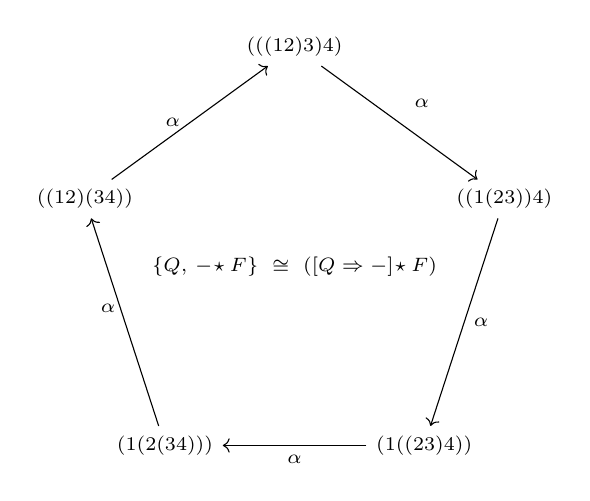
\begin{tikzpicture}[scale=1.0, every node/.style={font=\scriptsize}]
  % radius
  \def\R{2.8}
  % vertices
  \node (v1) at (90:\R)      {$(((12)3)4)$};
  \node (v2) at (18:\R)      {$((1(23))4)$};
  \node (v3) at (-54:\R)     {$(1((23)4))$};
  \node (v4) at (-126:\R)    {$(1(2(34)))$};
  \node (v5) at (162:\R)     {$((12)(34))$};
  % edges with Day associator labels
  \draw[->] (v1) -- node[above right, xshift=2pt, yshift=2pt] {$\alpha$} (v2);
  \draw[->] (v2) -- node[right] {$\alpha$} (v3);
  \draw[->] (v3) -- node[below] {$\alpha$} (v4);
  \draw[->] (v4) -- node[above left] {$\alpha$} (v5);
  \draw[->] (v5) -- node[left] {$\alpha$} (v1);
  % center Day-flow reminder
  \node at (0,0) {$\{Q,\,-\!\star F\}\ \cong\ ([Q\Rightarrow -]\!\star F)$};
\end{tikzpicture}
\caption{\textbf{Associahedron $K_3$ with Day flows.} Vertices are full parenthesizations of $1,2,3,4$ (shorthand for $X_1,\dots,X_4$). Each edge is a single Day–associator flip $\alpha$. Along any edge, the “Day flow” $\{Q,-\!\star F\}\cong([Q\Rightarrow -]\!\star F)$ matches the two routes in the Kan cube; after applying the associahedral hull $\mathsf{cl}$, the compiled value is rebracketing-invariant (Thm.~\ref{thm:assoc-BC}).}
\label{fig:K3-pentagon}
\end{figure}

\paragraph{Didactic point.}
This micro–case makes visible (i) how the Day associator mediates rebracketing (edge flips),
(ii) how the alternation isomorphism pushes $\{Q,-\}$ through composition, and
(iii) how closure $\mathsf{cl}$ restores equality globally—while any pre-closure defect is
edge-local and therefore diagnosable (horn localization in \S\ref{subsec:alg-diagnostics}).

%------------------------------------------------------------
\subsection{Handoff to the residual compiler}
\label{subsec:handoff}

\paragraph{Compiled kernels (what to use).}
In conic/ellipsoidal modalities, \S\ref{sec:residual-compiler-conic} provides
closed-form residuals that collapse inner maximizations to a single conic layer.
Use these as \emph{Day kernels} for module composition:
\begin{itemize}[leftmargin=*, itemsep=.3ex]
\item \textbf{Linear objective on an ellipsoid} (Theorem~\ref{thm:ellipsoid-objective}):
\(
(Q\resid P)(a)=r(a)+\rho\|C^{-T}s(a)\|_2
\)
\;—\;SOCP epigraph.
\item \textbf{Robust linear constraint on an ellipsoid} (Theorem~\ref{thm:ellipsoid-constraint}):
\(
\sup_{\|Cb\|\le\rho}\langle s(a),b\rangle\le \gamma(a)
\iff
\rho\|C^{-T}s(a)\|_2\le \gamma(a)
\)
\;—\;SOCP.
\item \textbf{Concave quadratic in the uncertain variable} (S-lemma form in \S\ref{sec:residual-compiler-conic}):
single SDP via a scalar $\lambda\ge 0$ and the LMI in the theorem statement.
\item \textbf{KR/Wasserstein–1} (Eq.~\eqref{eq:kr-residual}):
\(
(Q\resid P)(a)=\mathbb E_{\widehat{\mathsf P}}[h(a,\xi)]+\rho\,L_a
\)
\;—\;first-order Lipschitz penalty.
\item \textbf{$\phi$–divergence} (Eq.~\eqref{eq:phi-dual-2p}, e.g.\ KL, $\chi^2$):
1D (KL) or closed-form ( $\chi^2$ ) residuals used as kernels.
\end{itemize}
Write the residualized module as $K_i^\sharp := Q\multimap K_i$ and cache its conic
epigraph (SOCP/SDP) for reuse.

\paragraph{Composition-stable envelopes (what it guarantees).}
By Theorem~\ref{thm:comp-sion} and Theorem~\ref{thm:assoc-BC}, for any stack
$K=K_1\star\cdots\star K_m$ and payload $F$,
\[
\mathsf{cl}\,\{Q,\,K\star F\}
\ \cong\
\mathsf{cl}\Big(\ (K_1^\sharp\star\cdots\star K_m^\sharp)\star F\ \Big),
\]
and this value is \emph{independent of the parenthesization} of the $K_i$.
Moreover, $\mathsf{cl}$ is lax–monoidal (Lemma~\ref{lem:lax-monoidal-hull}), so
\emph{convexify–then–compose} is never stronger than \emph{compose–then–convexify}
(Minkowski-type subadditivity).

\paragraph{Complexity and solver footprint.}
In the ellipsoidal/conic cases, the compiled objective is a \emph{single} SOCP/SDP
per instance (see Example~\ref{ex:compiled-socp}). Compared to bilevel schemes with
inner trust-region/QCQP oracles, Theorem~\ref{thm:conic-speedup} shows a per-iteration
speedup by removing $\Omega(\sum_i d_i^{\,\omega}\log(1/\varepsilon))$ inner work,
eliminating inner–outer tolerance coupling and improving numerical robustness.

\paragraph{Practice (how to run it).}
\begin{enumerate}[leftmargin=*, itemsep=.35ex]
\item \textbf{Compile each primitive to a kernel.} For every module $K_i$, build
$K_i^\sharp=Q\multimap K_i$ using the closed forms above; store its SOCP/SDP epigraph.
\item \textbf{Assemble via Day, no parentheses.} Form
$K^\sharp:=K_1^\sharp\star\cdots\star K_m^\sharp$. Do not fix a bracketing; Day handles this.
\item \textbf{Apply the hull once.} Solve the single compiled envelope
$\mathsf{cl}(K^\sharp\star F)$ (one SOCP/SDP per instance in conic settings).
\item \textbf{Monitor interfaces.} Evaluate the BC-gap and flip-gaps
(\S\ref{subsec:alg-diagnostics}) around a baseline parenthesization; large local gaps
identify interfaces to refine (payload convexity, continuity, uncertainty class).
\item \textbf{Incremental updates.} When a local fix is made, only recompile the affected
$K_i^\sharp$ and update $K^\sharp$ by a few Day convolutions; the rest is unchanged.
\end{enumerate}

\paragraph{Notes on numerics.}
Use consistent barrier/tolerance settings across runs so that BC-gap differences reflect
model/interface effects rather than solver noise; prefer epigraph formulations (SOCP/SDP)
to prevent cancellation; cache factorizations for repeated kernels.

\paragraph{Takeaway.}
The categorical compilation (\S\ref{subsec:kan-through-day}, \S\ref{subsec:assoc-BC},
\S\ref{subsec:comp-bc-sion}) turns modular, possibly alternating pipelines into a single,
composition-stable envelope. The residual compiler in \S\ref{sec:residual-compiler-conic}
supplies the concrete SOCP/SDP/KR/$\phi$ kernels that make the approach practical at scale.

\section*{Declarations}

\noindent\textbf{Funding.}
No external funding was received for this work.

\medskip
\noindent\textbf{Competing interests.}
The author declares no competing interests.

\medskip
\noindent\textbf{Author contributions.}
Sole author: conceptualization, methodology, formal analysis, and writing.

\medskip
\noindent\textbf{Acknowledgments.}
The author used large language models for drafting, proofing, and \LaTeX{} formatting assistance, and for critical review suggestions: ChatGPT (GPT-5) and Grok 4 Fast. 
The author is responsible for the content and any errors.

\medskip
\noindent\textbf{License.}
This preprint is distributed under the Creative Commons Attribution 4.0 International (CC BY 4.0) license.

\bibliographystyle{plainnat}
\bibliography{QuantCompConvex}

\end{document}